\documentclass[11pt,a4paper]{article}

% Editorial submission layout using the standard article class.
% A Springer Nature template-compatible variant is retained separately.
\usepackage{graphicx}
\usepackage{amsmath,amssymb,amsfonts}
\usepackage{booktabs}
\usepackage{xcolor}
\usepackage{textcomp}
\usepackage{placeins}
\usepackage{xurl}
\usepackage[numbers,sort&compress]{natbib}
\usepackage[font=small,labelfont=bf]{caption}
\usepackage[hidelinks]{hyperref}

\raggedbottom
\setlength{\emergencystretch}{2em}
\usepackage[a4paper,left=24mm,right=24mm,top=22mm,bottom=22mm,footskip=10mm]{geometry}
\setlength{\parindent}{0pt}
\setlength{\parskip}{0.5em plus 0.08em minus 0.05em}
\setlength{\bibsep}{0.35em}
\setlength{\textfloatsep}{14pt plus 2pt minus 2pt}
\setlength{\floatsep}{12pt plus 2pt minus 2pt}
\renewcommand{\topfraction}{0.9}
\renewcommand{\bottomfraction}{0.8}
\renewcommand{\textfraction}{0.08}
\renewcommand{\floatpagefraction}{0.82}
\setcounter{secnumdepth}{0}
\pagestyle{plain}

\newcommand{\Htwo}{H$_2$}
\newcommand{\cnykg}{CNY\,kg$^{-1}$}
\newcommand{\cnykwh}{CNY\,kWh$^{-1}$}
\newcommand{\lowreturn}{approximately 1.45\%}

\begin{document}

\title{Curtailment traps early green hydrogen assets beyond the reach of learning}
\author{Jinwei Liang$^{1,\dagger}$, Zhiling Guo$^{2}$ and Haoran Zhang$^{1,*,\dagger}$\\[0.65em]
\small $^{1}$School of Urban Planning and Design, Peking University Shenzhen Graduate School,\\
\small Shenzhen, Guangdong, China\\
\small $^{2}$Department of Building Environment and Energy Engineering,\\
\small The Hong Kong Polytechnic University, Hong Kong, China\\[0.45em]
\small $^{*}$Corresponding author: \href{mailto:h.zhang@pku.edu.cn}{h.zhang@pku.edu.cn}\\
\small $^{\dagger}$These authors contributed equally to this work.}
\date{}

\maketitle

\begin{abstract}
Green hydrogen is expected to allow early electrolysis plants to inherit industry-wide cost declines through replaceable stacks. We test this channel using 10,214 Chinese wind and utility-scale solar records coupled to reconstructed hourly low-opportunity-cost electricity, six ERA5 weather-year replays and 30-year nominal equity cash flows. Two obstacles compound. Curtailment lowers electricity cost but concentrates operation, so 701 of 710 marginal records never reach the 60,000-h replacement threshold. More fundamentally, even where replacement occurs, the replaceable stack embodies only 18.2\% (range 11.3--42.3\%) of the capital saving achieved by a 2060 new build, and across a 1--10\% return frontier sector learning repairs marginal returns only where the initial shortfall is small. Price convergence deepens the loss but is not required. Replaceability is therefore neither sufficient nor decisive, and durable de-risking depends less on deployment volume than on verifiable power-supply commitment and pre-investment capacity flexibility before capital becomes irreversible.
\end{abstract}

\noindent\textbf{Keywords:} green hydrogen; low-opportunity-cost electricity; project finance; learning curves; vintage capital; investment flexibility
\vspace{1em}

Green hydrogen is central to deep decarbonisation in steel, chemicals, refining and long-distance transport\cite{staffell2019,yang2022,ueckerdt2021}. The International Energy Agency's net-zero pathway requires low-emissions hydrogen production to rise from about 1\,Mt today to roughly 70\,Mt by 2030, while the 2024 project pipeline contained nearly 520\,GW of announced electrolysers but only 4\% had reached final investment decision or construction\cite{iea2023nze,iea2024}. IRENA estimates that green-hydrogen production and infrastructure require cumulative investment of about US\$3.8 trillion by 2050\cite{irena2023}. China accounted for more than 40\% of electrolysis capacity reaching final investment decision during the preceding year and 60\% of manufacturing capacity\cite{nea2024capacity,pan2021,guo2023coal,ndrc2022}.

Embodied technical change provides the natural starting point. In vintage-capital theory, improvements embodied in new equipment do not automatically raise sunk-capital productivity\cite{solow1960}. Experience-curve evidence and deployment models represent cost decline as a sector-level trajectory\cite{wright1936,arrow1962,mcdonald2001,nemet2006,ferioli2009,rubin2015,farmer2016,way2022,schmidt2017,brandt2024,song2021,glenk2023,irena2020,doe2024,worldbank2026,odenweller2022,zeyen2023,odenweller2025}. Electrolysis is an unusually permissive test because the stack accounts for 20--50\% of direct capital expenditure and is replaceable after tens of thousands of operating hours. Later stack cost, efficiency and lifetime gains can therefore enter an incumbent plant at replacement. Asset appraisal nevertheless needs vintage-specific incidence. The unresolved question is how much sector decline an already commissioned asset can physically capture.

Curtailment creates a conflict between entry cost and access to learning\cite{glenk2019,fan2025,nea2025hydrogen}. Low-opportunity-cost electricity can make electrolysis appear attractive at commitment, yet its temporal scarcity suppresses annual operating hours. Those hours determine whether a stack reaches its replacement threshold within the project life and hence whether later cost, efficiency and lifetime improvements enter the cash flow. The same resource condition that lowers the initial electricity bill can sever the replacement-mediated route to subsequent learning. We term this the \emph{curtailment-learning trap}: sector learning succeeds, but a sparsely operated incumbent remains locked to its commissioning vintage. Price convergence can deepen the loss, but it is not required for the mechanism.

We test this mechanism by coupling 10,214 operating wind and utility-scale photovoltaic records with reconstructed hourly low-opportunity-cost electricity, electrolyser sizing, 30-year nominal equity cash flow and vintage-specific learning; six ERA5 years provide a meteorological replay. Two disclosed firm rules define a lower screening case and a 6.5\% comparison within a continuous 1--10\% return frontier\cite{changyuan2026,chinabond2026,huadian2025}. In the reference reconstruction, 710 records qualify only under the lower rule. Of these, 701 fail to reach the 60,000-h stack-replacement threshold, central operating learning raises only three above 6.5\% at constant hydrogen price, and favourable transfer of all contemporaneous non-stack savings raises the count to eight. The central decomposition assigns 18.2\% of a 2060 new-build capital saving to the replaceable stack, with a source-grounded boundary of 11.3--42.3\%. Utilisation, not deployment scale alone, is the gate through which later learning reaches an early asset.

\section*{Low-opportunity-cost electricity, rather than total renewable output, limits developable supply}

System-constrained electricity compresses the physical hydrogen boundary within the covered inventory to about 6\% of its full-output upper bound. The inventory contains 4,149 operating wind records and 6,065 operating utility-scale photovoltaic records, totalling approximately 629\,GW. It represents 72\% of June 2024 official all-wind-plus-centralised-photovoltaic capacity, or 53\% when distributed photovoltaics are included. Under the reference resource profile, the inventory produces about 1,109\,TWh, whereas the 2025-calibrated system-constrained quantity is 70.8\,TWh. At 55\,kWh\,kg$^{-1}$\,H$_2$, these mutually exclusive branches correspond to 20.2 and 1.29\,Mt\,H$_2$\,yr$^{-1}$. The latter is therefore an inventory-conditioned physical boundary, not an estimate of national green-hydrogen potential.

Temporal concentration further reduces operable scale, consistent with China's system-specific renewable curtailment\cite{guo2023grid}. Under the reference daily peak-shaving reconstruction, the median record has positive constrained electricity in approximately 1,300 hours, and the highest-output 10\% of those hours contain about 91\% of annual constrained energy (Fig.~\ref{fig:resource}b). Replaying six ERA5 weather years gives inventory-level potentials of 1.28--1.34\,Mt\,yr$^{-1}$ and pairwise Spearman correlations above 0.996 for record-level resource rankings (Fig.~\ref{fig:resource}d,e). Annual peak-shaving and proportional allocation conserve the same annual energy yet produce median active durations of approximately 460 and 5,180 hours. The annual quantity is calibrated, but its record-level and hourly allocation remains only partially identified.

Maximising nominal energy capture can over-size electrolysers. With a 30\% minimum-load constraint for alkaline electrolysis, nominal capture targets of 60\% and 90\% require approximately 31.7 and 64.3\,GW of electrolyser capacity and produce 0.75 and 1.08\,Mt\,H$_2$\,yr$^{-1}$. Extending the target to 100\% raises capacity to about 163\,GW, but the larger unit cannot remain above minimum load during many constrained hours and realised production declines to 0.78\,Mt\,yr$^{-1}$. The relevant physical quantity is therefore usable production from the hourly profile, rather than annual electricity capture alone (Fig.~\ref{fig:resource}c).

Economic screening retains only part of this physical boundary. In the static 28~\cnykg{} reference, the lower firm rule qualifies 1,809 records over the 30-year primary horizon, corresponding to 8.4\,GW of electrolysers and 0.32\,Mt\,H$_2$\,yr$^{-1}$, or about one quarter of the constrained-electricity potential. Provincial physical potential is concentrated in Inner Mongolia, Xinjiang, Hebei, Gansu and Qinghai, but qualified supply does not scale proportionally with that potential (Fig.~\ref{fig:resource}a). Holding annual constrained energy fixed while changing only its hourly allocation moves qualified hydrogen supply from 0.12 to 0.81\,Mt\,yr$^{-1}$. Annual resource totals bound the opportunity; hourly concentration, minimum load and cash-flow conditions determine how much of it passes an economic screen.

\section*{Return criteria create a marginal band whose size depends on information at commitment}

Static price and technology expectations expose a continuous return frontier. At a producer-side price of 28~\cnykg{} with no future operating improvement credited at commitment, the lower rule qualifies 1,809 records and independent optimisation at 6.5\% qualifies 1,099. The remaining 710 records, 39\% of the lower-rule set, are \emph{strict-marginal}: some capacity has non-negative equity net present value (NPV) under the lower rule, but none reaches 6.5\%. Across 972 deterministic configurations, the qualified sets remain separated (Fig.~\ref{fig:admission}a). At the IEA's 2021 China utility-solar cost-of-capital estimate (4.9\% nominal), exact revaluation qualifies 1,255 records, compared with 1,036 at 8\% and 874 at 10\%\cite{ieacapital}. This is financing context rather than a green-hydrogen WACC; the cohort flow and full 1--10\% curve show that the band is not created by comparing only two thresholds (Fig.~\ref{fig:admission}b,c).

The lower rule expands project counts more than it expands hydrogen supply. Its 1,809 qualified records correspond to 8.4\,GW, 60.7\,billion CNY of gross installed-system capital and 0.32\,Mt\,H$_2$\,yr$^{-1}$. Strict-marginal records account for 1.5\,GW, 11.0\,billion CNY and 0.048\,Mt\,yr$^{-1}$, or 18\%, 18\% and 15\% of those totals. Xinjiang and Qinghai contain 393 strict-marginal records and approximately 68\% of their capital and 67\% of their output (Fig.~\ref{fig:admission}e); capacity--yield scaling confirms exposure across many small configurations (Fig.~\ref{fig:admission}f). These are plant-gate exposures. A provincial delivery-cost screen\cite{bi2026} contracts the two feasible sets to 331 and 93 records and completely changes strict-cohort membership (Supplementary Note 10); the spatial pattern therefore identifies production exposure, not delivered competitiveness.

Expected market conditions narrow the qualified set before investment, but do not remove the wedge between return requirements. If a linear producer-price path to 22~\cnykg{} and accessible operating learning are both known at commitment, 1,282 records qualify under the lower rule and 971 at 6.5\%, leaving 311 strict-marginal. With a linear path to 18~\cnykg{}, the corresponding counts are 1,077, 761 and 316; raising that anticipated-path criterion to 8\% and 10\% further reduces qualification to 625 and 474 records. Front-loaded and back-loaded paths at the same endpoints widen the lower-rule range to 849--1,482 records (Fig.~\ref{fig:admission}d). Thus, the static 1,809-record case is a rule-isolation counterfactual, not a prediction of investor behaviour.

Physical and temporal assumptions alter exact membership more than the separation. Daily peak-shaving, annual peak-shaving and proportional allocation yield 1,809, 475 and 5,544 lower-rule records and 710, 329 and 390 strict-marginal records, respectively (Extended Data Fig.~1a--c). A separate six-weather-year replay yields 2,315--2,682 lower-rule and 1,080--1,321 strict-marginal records on a common grid; none of its strict cohorts reaches 6.5\% under the linear 18~\cnykg{} path. Adding the exact 1-MW boundary and adaptive local search reproduces the final 1,809, 1,099 and 710 memberships (Extended Data Fig.~1e). Exact counts are reconstruction-dependent; persistence of the return separation is the cross-reconstruction result.

\section*{Replacement access is insufficient to convert sector learning into durable incumbent returns}

Low-cost operation delays access to later learning. Across 710 strict-marginal records, the median 6.5\% NPV shortfall is 18.5\% of initial capital and 30-year operation is 54,800 hours. With a 60,000-hour initial stack life, 701 never replace; only nine do so in 2052--2055 (Fig.~\ref{fig:learning}a). Positive learning gain and replacement coincide because cost, efficiency and life improvements enter only then. Among these nine, the median gain is 2.0\% of initial capital and closes 39\% of the initial gap; only three cross 6.5\% at a flat 28~\cnykg{} (Fig.~\ref{fig:learning}c). Sparse use blocks access, and the payoff usually remains insufficient.

Fixed-cadence tests separate access from sufficiency. All 710 records trigger replacement at 20,000--50,000 hours, yet only four or five meet 6.5\% under central learning and five to eight under the source-optimistic path (Fig.~\ref{fig:learning}e). At 60,000 hours, nine trigger and three meet 6.5\%; at 80,000--100,000 hours none triggers, and three pass only because they avoid replacement expenditure. Even a 90\% stack-cost learning rate combined with a 20,000-hour cadence closes only 39 gaps, leaving 671 unresolved. Cohort-wide reversal requires twenty-fold joint operating improvements and replacement every 20,000--30,000 hours; at 60,000 hours only six upgrade. Across 55 lower-to-higher return comparisons, all five cohorts with median initial gaps below 2\% of CAPEX upgrade at rates of 22.8--72.5\%, whereas the 24 cohorts with gaps of at least 10\% average 0.43\% and never exceed 2.66\% (Fig.~\ref{fig:learning}f). Reversal is therefore possible, but only where the initial shortfall is already commensurate with the limited gain that can reach an incumbent.

Component incidence further limits how much sector learning can enter an existing plant. The central decomposition assigns 67.5\% of installed cost to direct CAPEX and 25\% of direct CAPEX to the stack. On that basis, the replaceable stack embodies 18.2\% of the capital saving achieved by a 2060 new build; crossing source-grounded component shares and three conditional learning paths gives a range of 11.3--42.3\% (Fig.~\ref{fig:learning}b). We then credit the incumbent, at its first replacement, with up to 100\% of the contemporaneously available non-stack saving without tax, retrofit cost or repetition. Under a flat 28~\cnykg{} price, this deliberately favourable transfer raises the number crossing 6.5\% from three to eight; across the full component boundary the range is five to eight, leaving at least 702 records unresolved (Supplementary Note 5). Price decline is therefore not required for the vintage separation.

Price convergence dominates post-entry survival. At a 2060 endpoint of 22~\cnykg{}, front-loaded, linear and back-loaded paths leave 4, 45 and 298 strict-marginal records above the lower criterion; none reaches 6.5\%. At 18~\cnykg{}, the corresponding counts are 0, 0 and 102. The linear-path terminal price required for a strict-marginal record to reach 6.5\% has a median of 38.2~\cnykg{} and a 5th--95th percentile range of 33.1--42.2~\cnykg{} (Fig.~\ref{fig:learning}d). Relative to the flat-price, no-learning counterfactual, a linear path to 18~\cnykg{} removes 5.31\,billion CNY from cohort NPV at the lower criterion, whereas operating learning restores only 4.7\,million CNY, or 0.09\% of that loss (Supplementary Note 5). Vintage incidence explains why incumbents cannot capture enough compensation even at constant price; conditional price convergence determines the magnitude of subsequent loss. Under declared priors, joint propagation leaves approximately 0.04\% of project--draw pairs above 6.5\% (0.02--0.09\% across tests), an assumption-weighted rather than empirical probability (Supplementary Note 11).

\section*{Price-informed screening and capacity flexibility move risk before capital lock-in}

Separating expectations at commitment from conditions realised afterwards changes the apparent value of a lower return rule. If the static 28~\cnykg{} lower-rule capacities are committed and the producer price subsequently follows a linear path to 18~\cnykg{}, only 274 of 1,809 records remain above 6.5\%; 44.0 of 60.7\,billion CNY falls below that criterion and durable output is 0.103\,Mt\,H$_2$\,yr$^{-1}$. If the same price and operating-learning path is anticipated at commitment, the lower rule qualifies 1,077 records rather than 1,809. Requiring 6.5\% under that anticipated path retains 761 records, 18.4\,billion CNY and 0.120\,Mt\,yr$^{-1}$ (Fig.~\ref{fig:screening}b). Relative to static lower-rule entry, this screen commits 70\% less capital while retaining 16\% more output that remains above 6.5\% under the realised path.

A higher static criterion alone does not substitute for forward information. The static 6.5\% rule selects 1,099 records, but only 490 remain above 6.5\% under the linear 18~\cnykg{} path and 10.4 of 33.1\,billion CNY becomes exposed. A screen robust to all three timing shapes at the 18~\cnykg{} endpoint retains 408 records, 8.6\,billion CNY and 0.060\,Mt\,yr$^{-1}$; at 22~\cnykg{}, the corresponding linear and timing-robust screens retain 971 and 781 records (Fig.~\ref{fig:screening}a,f). Zero non-durable exposure is imposed by these screens, so the scientifically informative quantities are the capital and supply that survive each information requirement, not the zero itself.

Pre-investment capacity flexibility converts resource error into avoided commitment rather than post-investment loss. Holding the static 28~\cnykg{} producer price and no-learning conditions used at entry fixed, 75\% realisation of the low-cost electricity assumed at design leaves 157 locked-capacity records and 1.18\,billion CNY below the lower criterion while producing 0.292\,Mt\,H$_2$\,yr$^{-1}$; 325 records, contributing 0.105\,Mt\,yr$^{-1}$, reach 6.5\%. Under continuous downsizing without a minimum-build cutoff, each additional 25 percentage points of adjustability leaves the same 3.93\,billion CNY of planned CAPEX uncommitted. The first increment reduces exposure to 99 records and 0.61\,billion CNY while retaining 0.280\,Mt\,yr$^{-1}$, of which 0.145\,Mt comes from records reaching 6.5\%; at 50\% adjustability, exposure is eliminated and 7.86\,billion CNY, or 12.9\% of initially selected capital, remains uncommitted. Although total output then falls only to 0.267\,Mt\,yr$^{-1}$, 91.3\% of the locked outcome, output from the 656 records reaching 6.5\% rises from 0.105 to 0.169\,Mt\,yr$^{-1}$, 60\% above the locked case. Across the four equal capital increments, additional records reaching 6.5\% decline from 178 to 127, reducing the marginal durability yield from 45.3 to 32.3 records per CNY billion not committed (Fig.~\ref{fig:screening}e,g). Flexibility therefore sheds capital faster than production. Under the primary 1-MW engineering convention, 25\% adjustability instead maps 154 sub-threshold capacities to no-build and mechanically reports zero exposure (Fig.~\ref{fig:screening}d). The option value is robust, but the adjustment share at which exposure reaches zero depends on minimum viable project scale and is not a universal 25\% threshold.

Retrospective support is much larger than the illustrative policy limits tested. Under the linear 18~\cnykg{} path, no strict-marginal record is upgraded by either a 4~\cnykg{} 15-year producer premium or a 25\% upfront capital grant. The median requirements are 8.8~\cnykg{} and 44.5\%, and even the least costly record requires more than the two illustrative limits (Fig.~\ref{fig:screening}c). These are plant-gate financing gaps: a China-specific delivery-cost transfer replaces the strict cohort entirely, and the delivery-exposed prior produces no upgrade. Route and offtake screening must therefore precede instrument design. Forward screening and capacity flexibility act on the source of production-side exposure, whereas ex post support finances a return gap after the capital configuration has been fixed.

\section*{Discussion}

The curtailment-learning trap refines the vintage-capital test from whether a component is replaceable to whether replacement occurs within the economic life of the asset. A replaceable stack is only a potential conduit for embodied technical change. In the reference cohort, sparse operation leaves 701 of 710 strict-marginal records below the 60,000-h trigger; among the nine that replace, central learning closes only three return gaps at constant price. Forcing all 710 records to replace every 20,000--50,000 hours removes the access constraint, yet central learning still raises only four or five above 6.5\%, and a source-optimistic path raises five to eight. Even a 90\% stack-cost learning rate with 20,000-h replacement closes only 39 gaps. Replaceability is therefore necessary but not sufficient: utilisation first governs access, and the limited share of learning embodied in the replacement then governs sufficiency. Green hydrogen is not an exception to embodied technical change, but a sharp case in which the operational use of a component determines whether its new vintage ever arrives.

This distinction shifts effective de-risking towards information available before capital becomes irreversible\cite{majd1987,pindyck1991}. Capacity support does not ensure that incumbent stacks accumulate the hours needed to receive later improvements. Verifiable low-cost operating-hour commitments, through long-term power contracts, guaranteed operating windows or stable loads, are therefore better aligned with the mechanism than installed capacity alone. Under a linear price path to 18~\cnykg{}, a path-informed 6.5\% screen commits 70\% less capital than static lower-rule entry while retaining 16\% more output above the comparator. When 75\% of designed low-cost electricity is realised, continuous 50\% pre-investment adjustment withholds 7.86\,billion CNY and retains 91\% of locked-case output, while increasing output from configurations above 6.5\% by 60\%. These results favour credible utilisation and capacity flexibility before final investment decision, rather than assuming later deployment repairs a low-use asset.

The non-random inventory and reconstructed hourly allocation yield conditional exposure, not national potential, although six ERA5 replays preserve resource ranking. Hydrogen is valued at the plant gate with full sales; transport, storage, local demand and basin-level water constraints can reduce feasible membership, especially in Xinjiang and Qinghai\cite{beswick2021,irenawater2023}. Buffering or transmission could raise utilisation and reopen the replacement channel, while different degradation physics could weaken the link between hours and replacement. The firm rules are screening scenarios rather than national policy or estimates of equity cost, and 6.5\% is a comparator rather than a break-even condition. The mechanism remains: sector learning reaches an incumbent only through changes within its own operating and replacement history.

\section*{Methods}

\subsection*{Research design and system boundary}

The analysis unit is an operating wind or utility-scale photovoltaic \texttt{ObjectId} record in the project inventory. Resource reconstruction, capacity candidates, nominal equity cash flow, entry and durability are evaluated at record level before provincial and inventory-level aggregation. Separate construction phases of one named facility can appear as multiple records, so all counts are described as project records rather than distinct physical plants. The primary financial horizon contains 30 operating years, from 2026 through 2055; 15-, 20-, 25- and 35-year horizons are sensitivity cases. Conditional market and learning paths are specified through 2060 to retain a common endpoint, but only values realised through 2055 enter the primary asset cash flow. Continued access to low-cost electricity represents contract renewal, host repowering or replacement supply. The primary branch uses system-constrained electricity. A mutually exclusive full-output branch redirects all modelled renewable output to electrolysis and charges the provincial feed-in price as an opportunity-cost proxy, providing a physical diversion boundary.

The financial boundary includes the installed electrolysis system: electrolyser package, rectification and electrical systems, gas--liquid separation and purification, cooling, water treatment, buildings, engineering, procurement, construction and contingency. It excludes the existing renewable host asset, off-site compression and storage, hydrogen pipelines, distribution and end-use facilities. Construction period, working capital and residual value are zero in the primary boundary, and all hydrogen is sold at the producer side. Separate tests add zero to two construction years with capitalised interest and after-tax residual values of 0--20\% of initial capital. These choices define the production-side investment boundary.

\subsection*{Project inventory and hourly low-opportunity-cost electricity}

The inventory combines the June 2024 Global Wind Power Tracker and Global Solar Power Tracker releases and contains 10,214 operating records with capacity, technology, coordinates and province\cite{gem2024}. The 2020 hourly reference files are research-group station-level model outputs previously used and documented by Li and Zhang\cite{li2026}, and are reused here; that article describes simulated generation records and reconstructs hourly curtailment by daily peak-shaving to provincial rates. The files contain 8,784 leap-year hours and 15,573 unique identifiers, of which all 10,214 inventory identifiers match one-to-one. We sum the grid-delivered and constrained components only to recover a pre-allocation full-output shape; neither the earlier study's projected 2030 curtailment rates nor its hourly constrained quantities enter our annual calibration. We instead calibrate annual constrained energy to 2025 province- and technology-specific utilisation rates\cite{renewable2025}. A separate 42-cell comparison with public monthly monitoring data supports seasonal utilisation magnitudes but does not identify hourly event timing\cite{renewablemonthly}. For province $p$ and technology $s$, the annual constrained share is $r_{ps}=1-U_{ps}$. The reference daily peak-shaving reconstruction solves a threshold $\theta_{id}$ for record $i$ and day $d$:

\begin{equation}
r_{ps}=1-U_{ps}, \qquad
\sum_{h=1}^{24}\max\!\left(P_{idh}-\theta_{id},0\right)
=r_{p(i)s(i)}\sum_{h=1}^{24}P_{idh},
\label{eq:curtailment}
\end{equation}
where $P_{idh}$ is calibrated full output. The reference reconstruction applies $r_{ps}$ uniformly to records within each province--technology group; record-level allocation is treated as partially identified. Two concentration extremes therefore allocate the same group total greedily to records in ascending or descending installed-capacity order, capped by each record's full output. All three allocations conserve every group total exactly. The hourly proxy is $C_{idh}=\max(P_{idh}-\theta_{id},0)$; thresholds are solved by bisection and annual energy is rescaled exactly. Annual peak-shaving uses one threshold over the annual duration curve, whereas proportional allocation assigns the constrained share at every hour. The resulting inputs are modelled generation and allocation profiles used to test the investment mechanism.

Weather-year sensitivity uses ERA5 hourly 100-m wind components, 2-m temperature, surface pressure and surface solar radiation downwards for 2020--2025\cite{hersbach2020,era5data}. Variables are bilinearly interpolated to each record. Wind output uses an air-density-corrected generic power curve, and photovoltaic output uses a temperature-corrected irradiance model. Each record is calibrated to its 2020 reference equivalent full-load hours; this scalar is fixed in later weather years so that replay changes meteorological shape while holding the 2025 utilisation-rate calibration constant.

Figure~\ref{fig:resource}a separates the analytical main map from its locator inset. The main-map land mask, coastline and visible national and provincial linework use OpenStreetMap coastline polygons and administrative relations\cite{osmcoast}. Records and all main-map layers use the same China Albers equal-area projection. The boxed South China Sea locator is a cleaned display derivative of the Ministry of Natural Resources standard-map product GS(2023)2767\cite{mnrmap2023}; it is not used for masking, spatial assignment or any numerical result. Both sources provide cartographic context rather than legal adjudication. Query timestamps, product identifiers, transformations and integrity hashes are archived with the figure data.

\subsection*{Electrolyser dispatch and capacity choice}

For candidate electrolyser capacity $K$, the plant operates only when available low-opportunity-cost power exceeds the minimum-load fraction $\lambda K$. Absorbed power in hour $t$ is

\begin{equation}
A_{it}(K)=\mathbb{1}\!\left(C_{it}\geq\lambda K\right)\min(C_{it},K).
\label{eq:dispatch}
\end{equation}
Annual absorbed electricity, operating hours and hydrogen output are

\begin{equation}
\begin{aligned}
E_i(K)&=\sum_t A_{it}(K)\Delta t,\\
h_i(K)&=\sum_t\mathbb{1}\!\left(A_{it}>0\right)\Delta t,\\
H_{iy}(K)&=1000\sum_t\frac{A_{it}(K)\Delta t}{\varepsilon_{iyt}}.
\end{aligned}
\label{eq:operation}
\end{equation}
Here $\Delta t=1$\,h, $E_i$ is measured in MWh, $h_i$ in hours and $H_{iy}$ in kg; the factor 1000 converts MWh to kWh. The alkaline main case uses $\lambda=0.30$. Candidate capacities are generated from 128 nested resource-capture fractions, with the exact 1-MW engineering lower bound added as an independent candidate. Candidates below 1\,MW or with zero production are removed. For return criterion $r$, every record is independently resized by

\begin{equation}
K_i^*(r)=\underset{K\in\mathcal{K}_i,\,K\geq1\,\mathrm{MW}}{\operatorname{arg\,max}}
\;\mathrm{NPV}_i(K;r).
\label{eq:capacity}
\end{equation}
A strict-marginal record has at least one capacity with non-negative NPV at the low criterion and no capacity with non-negative NPV at 6.5\%. Grid density, the 1-MW boundary, continuous local search, lower minimum loads and proton-exchange membrane (PEM) operation are assessed in the Supplementary Information. Dispatch is directly coupled without a battery or hydrogen buffer, so the minimum-load and oversizing results describe the unbuffered operating configuration.

\subsection*{Installed-system cost, nominal equity cash flow and return criteria}

For capacity $K_i$ in MW and installed-system unit cost $c_{\mathrm{sys}}$ in CNY\,kW$^{-1}$, initial investment, debt and equity are

\begin{equation}
I_i=1000K_i c_{\mathrm{sys}}, \qquad
D_{i0}=\delta I_i, \qquad
Eq_{i0}=(1-\delta)I_i,
\label{eq:investment}
\end{equation}
where $\delta$ is the debt share. The World Bank reports 500--1,500\,USD\,kW$^{-1}$ for installed alkaline systems; using a transparent conversion assumption of 7.2\,CNY per USD gives deterministic bounds of 3,600 and 10,800\,CNY\,kW$^{-1}$, with 7,200\,CNY\,kW$^{-1}$ as the midpoint central case\cite{worldbank2026}. The IEA's 600--1,200\,USD\,kW$^{-1}$ China interval provides contextual equipment-cost evidence, while the World Bank interval defines the installed-system boundary used here\cite{iea2025}. Fixed operations and maintenance (O\&M) is 5\% of initial capital per year, and an explicit stack replacement costs 11\% when triggered\cite{doe2024}. Mutually exclusive all-in operating-cost conventions are tested to avoid double counting\cite{worldbank2026}. Constrained electricity costs 0.10~\cnykwh{} centrally and 0--0.20~\cnykwh{} in sensitivity. Water uses provincial values reported in Supplementary Table 3 of the earlier study\cite{li2026} and 15\,kg of water per kg H$_2$ centrally, with 10--60\,kg\,kg$^{-1}$ tested as a direct-cost boundary.

All model price and cost scenarios are expressed in constant 2026 CNY and converted to nominal cash flow using a common escalation rate $\pi$. The 28~\cnykg{} entry reference is anchored numerically to the December 2024 cross-route producer sample:

\begin{equation}
X_y^{\mathrm{nom}}=X_y^{\mathrm{real}}(1+\pi)^{y-2026}, \qquad
R_{iy}=H_{iy}P_y(1+\pi)^{y-2026}.
\label{eq:nominal}
\end{equation}
The central accounting case uses $\pi=2\%$ and tests 0\%, 1\% and 3\%. Nominal loan rates and nominal return criteria are applied only to nominal cash flows. The central financing structure is 70\% debt, a 3.5\% nominal loan rate, a 15-year term and two years of principal grace. Corporate income tax is 25\% and tax losses can be carried forward for five years\cite{taxlaw}; a ten-year straight-line depreciation schedule is a transparent accounting assumption applied to initial and replacement capital.

Annual free cash flow to equity subtracts operations, stack replacement, tax, interest and principal from revenue. Classification is based on NPV consistency because replacement expenditure can create multiple cash-flow sign changes:

\begin{equation}
\begin{aligned}
CF^{Eq}_{iy}&=R_{iy}-O_{iy}-M_{iy}-T_{iy}-Int_{iy}-Prin_{iy},\\
\mathrm{NPV}_i(K;r)&=-Eq_{i0}+\sum_{y=1}^{Y}\frac{CF^{Eq}_{iy}}{(1+r)^y}.
\end{aligned}
\label{eq:npv}
\end{equation}
A record passes criterion $r$ when the NPV of its criterion-specific optimum is non-negative. ``Durable 6.5\%'' means that the locked 2026 investment and capacity produce non-negative 30-year equity NPV at both the lower rule and 6.5\%. Capacity remains fixed after construction, and classification uses equity value without debt-service-coverage, reserve-account or default tests. It is therefore a return-screen classification, not a bankability test or prediction of actual investment.

We operationalise CHN Energy Changyuan's 2026 rule with the mean nominal five-year ChinaBond government bond yield over 20 trading days from 4 June to 2 July 2026, reported as approximately 1.45\%\cite{changyuan2026,chinabond2026}. ``Five-year'' denotes bond maturity, and the unrounded arithmetic mean is retained in the machine-readable calculation. The 6.5\% comparator comes from Huadian Energy's separate 2025 rule for hydrogen-based energy\cite{huadian2025}. These publicly disclosed firm-level criteria define an institutional scenario comparison; the lower value is not treated as a risk-adjusted cost of equity. We additionally scan nominal equity criteria from 1 to 10\% in 0.25-percentage-point increments.

To test whether the learning result is mechanically tied to either firm rule, we construct a dense return-screen surface under the flat 28~\cnykg{} reference. Eleven nominal criteria (approximately 1.45\%, 2\%, 3\%, 4\%, 5\%, 6\%, 6.5\%, 7\%, 8\%, 9\% and 10\%) generate all 55 lower-to-higher comparisons. Capacities are selected under each lower criterion without crediting future operating improvement, locked, and then revalued after central operating learning at every higher criterion. None of these pairs is interpreted as a representative weighted average cost of capital.

\subsection*{Vintage-specific operating learning and price paths}

The initial alkaline-stack electricity use is $\varepsilon_0=55$\,kWh\,kg$^{-1}$\,H$_2$ and stack life is 60,000 operating hours. Within-stack degradation is represented by

\begin{equation}
\varepsilon(a)=\varepsilon_0(1+\gamma a), \qquad
\gamma=\frac{2(57.3/55-1)}{60000},
\label{eq:degradation}
\end{equation}
so average lifetime electricity use is 57.3\,kWh\,kg$^{-1}$\,H$_2$. An operating asset receives improved efficiency, life and replacement cost only when a stack replacement is triggered by cumulative operating hours. Manufacturing learning in complete systems and balance-of-plant/engineering affects future new investment and is never used to reduce the 2026 sunk capital or annual fixed O\&M of an existing plant.

The stack-cost experience curve is

\begin{equation}
c_{\mathrm{stack},t}=c_{\mathrm{stack},0}
\left(\frac{Q_t}{Q_0}\right)^{-b}, \qquad
b=\frac{-\ln(1-LR)}{\ln 2},
\label{eq:learning}
\end{equation}
where $Q_t$ is cumulative deployment and $LR$ is the learning rate. The central path starts at 4\,GW, a rounded end-2025 global installed-capacity anchor\cite{iea2025}. Author-defined conditional anchors, contextualised by published deployment ranges, then reach 140, 700, 1,400 and 2,200\,GW in 2030, 2040, 2050 and 2060. A 20-GW starting normaliser provides the anchor sensitivity. The central path applies an author-selected 13\% conditional experience rate to future equipment and replacement-stack cost and 5\% to future balance-of-plant and engineering; applying system-level evidence to replacement stacks is the vintage-transfer assumption tested by the model. Electricity use and stack life are bounded trajectories interpolated in log-deployment space: they move from 55 to 50\,kWh\,kg$^{-1}$\,H$_2$ and from 60,000 to 90,000 h by 2060\cite{glenk2023,doe2024,worldbank2026,iea2025}. The central replacement-stack cost factor reaches its imposed 0.55 floor in 2028 and remains there; an existing record obtains the applicable factor only in its actual replacement year.

Three incidence and falsification boundaries test whether the result follows from restricted learning assumptions. The World Bank distinguishes direct and indirect CAPEX, reports 65:35--70:30 direct-to-indirect shares for large greenfield projects and places the stack at 20--50\% of direct CAPEX\cite{worldbank2026}. We therefore use $d\in\{0.50,0.675,0.70\}$ and $q\in\{0.20,0.25,0.35,0.50\}$, with central values $d=0.675$ and $q=0.25$. Installed capital is decomposed into stack ($s_S=dq$), other direct equipment ($d-s_S$) and indirect balance-of-plant/engineering ($1-d$). The central $s_S=0.16875$ is a component-accounting share; the separate 11\% replacement-event expenditure remains a cash-flow assumption. The share of new-build capital savings embodied in the replaceable stack is
\begin{equation}
\phi_t=\frac{s_S(1-f^S_t)}{s_S(1-f^S_t)+(d-s_S)(1-f^E_t)+(1-d)(1-f^B_t)},
\label{eq:incidence}
\end{equation}
where $f^S_t$, $f^E_t$ and $f^B_t$ are the stack, other direct-equipment and indirect-capital cost factors. Under the central path, $\phi_{2060}=0.182$; the full component-share and learning-path boundary is 0.113--0.423. A deliberately favourable transfer boundary then credits an incumbent at its first stack replacement with
\begin{equation}
T_{it}=\lambda I_{i0}\left[(d-s_S)(1-f^E_t)+(1-d)(1-f^B_t)\right],
\qquad \lambda\in[0,1],
\label{eq:transfer}
\end{equation}
where $I_{i0}$ is initial installed-system CAPEX and $\lambda$ is evaluated in 0.01 increments. The transfer is added directly to equity cash flow without tax, retrofit cost or repetition, making it an upper bound rather than a proposed instrument. A reduced-form pass-through elasticity links future new-build cost to producer price,
\begin{equation}
I_t^{\mathrm{new}}=d f_t^E+(1-d)f_t^B,
\qquad P_t=28\left(I_t^{\mathrm{new}}\right)^\beta,
\qquad \beta\in\{0,0.25,0.50,0.75,1\}.
\label{eq:passthrough}
\end{equation}
This is an incidence boundary, not an estimated price elasticity or a supply--demand forecast. An auxiliary test separately scales incumbent access to electricity-use, stack-life and replacement-cost improvements from zero to the central path.

The stack-learning falsification boundary removes the 0.55 replacement-cost floor and scans the stack-cost learning rate from 0 to 90\% per doubling in one-percentage-point increments. It combines the central endogenous lifetime path with fixed replacement cadences of 20,000, 40,000, 60,000, 80,000 and 100,000 operating hours. The event replacement expenditure is separately varied from 6 to 45\% of installed capital. These tests ask how extreme learning strength, replacement frequency and replacement scope must become before the strict-marginal conclusion reverses; they are not forecasts of rational replacement policy.

Long-run hydrogen prices are conditional paths. For terminal price $P_{2060}$ and timing function $g_s$, the constant-2026-CNY price is

\begin{equation}
P_y=P_{2026}+(P_{2060}-P_{2026})g_s(\tau_y), \qquad
\tau_y=\frac{y-2026}{2060-2026}, \qquad
g_s\in\{\sqrt{\tau},\tau,\tau^2\},
\label{eq:price}
\end{equation}
where the three functions denote front-loaded, linear and back-loaded convergence. The initial price is 28~\cnykg{} and terminal values are 22, 18, 15 and 12~\cnykg{}. The endpoint is a conditional 2060 market anchor rather than the asset's terminal-year sale price; the primary project receives the corresponding path values only through 2055. Paired counterfactuals identify price and operating-learning contributions:

\begin{equation}
\begin{aligned}
\Delta\mathrm{NPV}_{\mathrm{price}}
&=\mathrm{NPV}(P_s,L_0)-\mathrm{NPV}(P_0,L_0),\\
\Delta\mathrm{NPV}_{\mathrm{learn}}
&=\mathrm{NPV}(P_s,L)-\mathrm{NPV}(P_s,L_0).
\end{aligned}
\label{eq:decomposition}
\end{equation}

We distinguish information available at commitment from subsequent realisation. The static reference uses a constant 28~\cnykg{} price and credits no future operating learning when capacity is selected; it isolates the effect of changing the return criterion under common contemporaneous assumptions. Twelve anticipated cases cross the four terminal prices and three timing shapes and allow the replacement-mediated operating path to enter the commitment calculation. An expectation--realisation matrix then evaluates capacities selected under static 28, anticipated 22-linear and anticipated 18-linear conditions against realised flat-28, 22-linear and 18-linear paths. No probability is assigned to these cases.

The reference lifetime calculation holds low-cost electricity equivalent hours at their 2025-calibrated level. A persistence audit scales annual active hours, absorbed electricity and electricity expenditure by a linear factor from 1 in 2026 to 0.50, 0.75, 1.00 or 1.25 in 2060, spanning declining and expanding contract-equivalent access.

\subsection*{Forward screening, capacity flexibility and support boundaries}

Forward screening places a long-run price endpoint and timing in the capacity-choice problem before FID and retains only capacities with non-negative NPV at both criteria. Timing-robust screening first selects the engineering-eligible capacity with the greatest worst-case 6.5\% NPV across $\mathcal{S}$, the front-loaded, linear and back-loaded paths:

\begin{align}
K_i^{\mathrm{rob}}&=\underset{K\in\mathcal{K}^{\mathrm{elig}}_i}{\operatorname{arg\,max}}
\;\min_{s\in\mathcal{S}}\mathrm{NPV}_i(K;6.5\%,s),
\label{eq:robustcapacity}\\
S_i^{\mathrm{rob}}&=\mathbb{1}\!\left[
\min_{s\in\mathcal{S}}\mathrm{NPV}_i(K_i^{\mathrm{rob}};6.5\%,s)\geq0\right]
\mathbb{1}\!\left[
\min_{s\in\mathcal{S}}\mathrm{NPV}_i(K_i^{\mathrm{rob}};r_{\mathrm{low}},s)\geq0\right].
\label{eq:robustscreen}
\end{align}

Here $\mathcal{K}^{\mathrm{elig}}_i$ is the engineering-eligible capacity set. A selected record is retained only when $S_i^{\mathrm{rob}}=1$, matching the implemented sequence of capacity selection followed by the two-criterion worst-case screen. A stricter minimax screen replaces $\mathcal{S}$ with the Cartesian product of the three timing shapes and terminal prices from 12 to 22~\cnykg{} in 1-CNY increments. Because project NPV is monotone in price, this endpoint-and-timing screen is governed by the 12~\cnykg{} boundary but is reported separately to make the information assumption explicit.

Capacity flexibility describes the share that can be adjusted before construction after a resource deviation is known. If $K_i^0$ is original capacity and $K_i^*(\rho)$ is the re-optimised capacity under resource realisation $\rho$, installed capacity at adjustability $a$ is

\begin{equation}
K_i(a,\rho)=K_i^0+a\left[K_i^*(\rho)-K_i^0\right],
\qquad a\in\{0,0.25,0.50,0.75,1\}.
\label{eq:flexibility}
\end{equation}
Among positive engineering-eligible capacities, $K_i^*(\rho)$ maximises low-criterion NPV. If none has non-negative NPV, $K_i^*(\rho)=0$, representing cancellation before commitment; the primary engineering convention also maps interpolated capacities below 1\,MW to zero. Because this rule can create a discontinuity, a separate M129 audit repeats the 75\% resource-realisation surface with minimum build sizes of 0, 0.1, 0.5, 1 and 2\,MW; the zero-bound case permits continuous downsizing and distinguishes economic exposure from threshold cancellation. Exposed capital is gross initial investment in positive-capacity records that cease to satisfy the low-return criterion after the resource deviation. Avoided capital is planned investment withheld through downsizing or cancellation. Complete flexibility assumes that resource error is resolved before FID and that capacity can be adjusted without cancellation, lead-time or interconnection costs. Support boundaries search for the minimum constant 2026--2040 producer-price premium or upfront capital grant that makes a locked strict-marginal record satisfy 6.5\%, yielding equivalent financing gaps for comparison with forward screening.

\subsection*{Robustness, uncertainty and quality control}

Deterministic robustness spans installed-system capital cost, constrained-electricity price, operating cost, resource realisation and persistence, debt share, nominal loan rate, escalation, evaluation horizon, minimum load, alkaline and PEM technology, learning intensity, learning-start anchor, terminal hydrogen price, construction duration, residual value, producer-side netback and electrical buffering. The constrained-electricity branch contains 972 factorial combinations, and a mutually exclusive full-output branch adds 324 opportunity-cost combinations, for 1,296 deterministic cases in total. All combinations have equal diagnostic status and define a robustness domain; their frequencies are not probabilities. Because empirical joint distributions are unavailable, a separate assumption-weighted propagation declares six alternative priors over terminal price, timing, operating learning, weather-year resource factors, price--learning dependence and delivery netback and uses 5,000 draws per prior case. These outputs quantify implications conditional on the declared priors rather than historically identified investment odds. Within each province--technology group, two annual-energy-conserving concentration extremes assign constrained energy first to smaller or larger records, respectively, partially identifying outcomes under the unknown allocation. The financing contribution to within-grid dispersion is evaluated over its specified parameter range. Netback penalties of 0--4~\cnykg{} are applied before reoptimising entry. Electrical buffers of zero to four equivalent hours are dispatched against the original hourly profiles; free lossless storage defines a physical upper bound, whereas costed cases include initial capital, fixed operation and maintenance, round-trip loss and periodic replacement.

Capacity discretisation is checked against 128- and 256-candidate nested grids and continuous local search. Weather shape is checked by replaying ERA5 2020--2025. In addition to the M129 resource check, the complete entry, learning and support calculations are replayed with a common 16-candidate grid for each weather year; these G16 counts are reported as a separate robustness experiment and are never pooled with the M129 main cohort. Set stability is measured by

\begin{equation}
J(A,B)=\frac{|A\cap B|}{|A\cup B|}.
\label{eq:jaccard}
\end{equation}
All figures and reported values are generated from record-level output tables. Automated checks cover annual energy conservation, cohort denominators, criterion nesting, nominal cash-flow reconstruction, capacity-search convergence and figure--text consistency. Provincial water price and constrained-electricity settlement are retained as transparent boundaries where evidence is insufficient for causal or implementation claims.

\section*{Data availability}

Redistributable project-inventory fields, annual utilisation inputs, processed ERA5 outputs, parameter-source registers, figure source data and result tables are maintained in the accompanying GitHub repository at \href{https://github.com/1223044298-ship-it/curtailment-traps-early-green-hydrogen-assets-beyond-the-reach-of-learning}{github.com/1223044298-ship-it/curtailment-traps-early-green-hydrogen-assets-beyond-the-reach-of-learning}. The repository is private during manuscript review. The manuscript-aligned revision is identified by a fixed Git commit, and repository access will be supplied to editors and reviewers; the accepted release will be made public and archived under a versioned DOI before publication. Source ERA5 variables are publicly available from the Copernicus Climate Data Store under its applicable terms. The 2020 monthly model-output files were generated within the authors' research group, previously used and documented by Li and Zhang\cite{li2026}, and reused here rather than generated specifically for the present study. Their provenance is fixed to that article and its \href{https://github.com/Lynn20001130/-hydrogen-blending-analysis/tree/43af9fef041a7c55ca154cc6a40c5d339c23c521}{public source-code repository at commit 43af9fe}. That source-study code reads, but does not distribute or regenerate, the underlying monthly files. The two 10,214-by-8,784 hourly profile arrays used here are deterministic derivatives of those files. The monthly files and derived arrays required for a clean raw-to-results rerun are not redistributed in the repository; they are held by the authors' research group and documented by filename, dimension, SHA-256 checksum, identifier matching, analytical role and transformation code. Requests for research access should be sent to the corresponding author at \href{mailto:h.zhang@pku.edu.cn}{h.zhang@pku.edu.cn} and should identify the intended research use; access is subject to contributor and institutional approval and applicable data-sharing conditions. These files are model outputs and are not represented as independently observed station dispatch.

\section*{Code availability}

Custom code for constrained-electricity reconstruction, ERA5 replay, electrolyser dispatch and capacity optimisation, nominal equity cash flow, learning-flip boundaries, forward screening, capacity flexibility and figure generation is maintained in the accompanying GitHub repository. The submission snapshot includes the software environment, execution order, input inventory and SHA-256 manifests. Packaged derived outputs support regeneration of all figures and numerical auditing of the reported results; a clean raw-to-results rerun additionally requires the request-access hourly inputs identified in \texttt{analysis\_code/INPUTS\_REQUIRED.csv}. No archival DOI has yet been assigned; the accepted public release will receive a versioned archival DOI before publication.

\begin{thebibliography}{99}

\bibitem{staffell2019}
Staffell, I. \emph{et al.} The role of hydrogen and fuel cells in the global energy system. \emph{Energy Environ. Sci.} \textbf{12}, 463--491 (2019). \href{https://doi.org/10.1039/C8EE01157E}{doi: 10.1039/C8EE01157E}.

\bibitem{yang2022}
Yang, X., Nielsen, C. P., Song, S. \& McElroy, M. B. Breaking the hard-to-abate bottleneck in China's path to carbon neutrality with clean hydrogen. \emph{Nat. Energy} \textbf{7}, 955--965 (2022). \href{https://doi.org/10.1038/s41560-022-01114-6}{doi: 10.1038/s41560-022-01114-6}.

\bibitem{ueckerdt2021}
Ueckerdt, F. \emph{et al.} Potential and risks of hydrogen-based e-fuels in climate change mitigation. \emph{Nat. Clim. Change} \textbf{11}, 384--393 (2021). \href{https://doi.org/10.1038/s41558-021-01032-7}{doi: 10.1038/s41558-021-01032-7}.

\bibitem{iea2023nze}
International Energy Agency. \emph{Hydrogen: Tracking Clean Energy Progress} (IEA, Paris, 2023). \href{https://www.iea.org/reports/hydrogen-2156}{Official analysis}.

\bibitem{iea2024}
International Energy Agency. \emph{Global Hydrogen Review 2024} (IEA, Paris, 2024). \href{https://www.iea.org/reports/global-hydrogen-review-2024}{Official report}.

\bibitem{irena2023}
International Renewable Energy Agency. \emph{World Energy Transitions Outlook 2023: 1.5$^{\circ}$C Pathway} (IRENA, Abu Dhabi, 2023). \href{https://www.irena.org/Publications/2023/Jun/World-Energy-Transitions-Outlook-2023}{Official report}.

\bibitem{nea2024capacity}
National Energy Administration. \emph{National Electric Power Industry Statistics and Photovoltaic Construction, January--June 2024} (20 and 25 July 2024, in Chinese). \href{https://www.nea.gov.cn/2024-07/20/c_1310782235.htm}{Power statistics}; \href{https://www.nea.gov.cn/2024-07/25/c_1310782757.htm}{photovoltaic breakdown}.

\bibitem{pan2021}
Pan, G., Gu, W., Hu, Q., Wang, J., Teng, F. \& Strbac, G. Cost and low-carbon competitiveness of electrolytic hydrogen in China. \emph{Energy Environ. Sci.} \textbf{14}, 4868--4881 (2021). \href{https://doi.org/10.1039/D1EE01840J}{doi: 10.1039/D1EE01840J}.

\bibitem{guo2023coal}
Guo, Y., Peng, L., Tian, J. \& Mauzerall, D. L. Deploying green hydrogen to decarbonize China's coal chemical sector. \emph{Nat. Commun.} \textbf{14}, 8104 (2023). \href{https://doi.org/10.1038/s41467-023-43540-4}{doi: 10.1038/s41467-023-43540-4}.

\bibitem{ndrc2022}
National Development and Reform Commission \& National Energy Administration. \emph{Medium- and Long-Term Plan for the Development of the Hydrogen Energy Industry (2021--2035)} (23 March 2022, in Chinese). \href{https://www.ndrc.gov.cn/xxgk/zcfb/ghwb/202203/t20220323_1320038.html}{Official plan}.

\bibitem{solow1960}
Solow, R. M. Investment and technical progress. In \emph{Mathematical Methods in the Social Sciences, 1959} (eds Arrow, K. J., Karlin, S. \& Suppes, P.) 89--104 (Stanford University Press, 1960). \href{https://www.econbiz.de/10002838822}{Catalogue record}.

\bibitem{wright1936}
Wright, T. P. Factors affecting the cost of airplanes. \emph{J. Aeronaut. Sci.} \textbf{3}, 122--128 (1936). \href{https://doi.org/10.2514/8.155}{doi: 10.2514/8.155}.

\bibitem{arrow1962}
Arrow, K. J. The economic implications of learning by doing. \emph{Rev. Econ. Stud.} \textbf{29}, 155--173 (1962). \href{https://doi.org/10.2307/2295952}{doi: 10.2307/2295952}.

\bibitem{mcdonald2001}
McDonald, A. \& Schrattenholzer, L. Learning rates for energy technologies. \emph{Energy Policy} \textbf{29}, 255--261 (2001). \href{https://doi.org/10.1016/S0301-4215(00)00122-1}{doi: 10.1016/S0301-4215(00)00122-1}.

\bibitem{nemet2006}
Nemet, G. F. Beyond the learning curve: factors influencing cost reductions in photovoltaics. \emph{Energy Policy} \textbf{34}, 3218--3232 (2006). \href{https://doi.org/10.1016/j.enpol.2005.06.020}{doi: 10.1016/j.enpol.2005.06.020}.

\bibitem{ferioli2009}
Ferioli, F., Schoots, K. \& van der Zwaan, B. C. C. Use and limitations of learning curves for energy technology policy: a component-learning hypothesis. \emph{Energy Policy} \textbf{37}, 2525--2535 (2009). \href{https://doi.org/10.1016/j.enpol.2008.10.043}{doi: 10.1016/j.enpol.2008.10.043}.

\bibitem{rubin2015}
Rubin, E. S., Azevedo, I. M. L., Jaramillo, P. \& Yeh, S. A review of learning rates for electricity supply technologies. \emph{Energy Policy} \textbf{86}, 198--218 (2015). \href{https://doi.org/10.1016/j.enpol.2015.06.011}{doi: 10.1016/j.enpol.2015.06.011}.

\bibitem{farmer2016}
Farmer, J. D. \& Lafond, F. How predictable is technological progress? \emph{Res. Policy} \textbf{45}, 647--665 (2016). \href{https://doi.org/10.1016/j.respol.2015.11.001}{doi: 10.1016/j.respol.2015.11.001}.

\bibitem{way2022}
Way, R., Ives, M. C., Mealy, P. \& Farmer, J. D. Empirically grounded technology forecasts and the energy transition. \emph{Joule} \textbf{6}, 2057--2082 (2022). \href{https://doi.org/10.1016/j.joule.2022.08.009}{doi: 10.1016/j.joule.2022.08.009}.

\bibitem{schmidt2017}
Schmidt, O., Gambhir, A., Staffell, I., Hawkes, A., Nelson, J. \& Few, S. Future cost and performance of water electrolysis: an expert elicitation study. \emph{Int. J. Hydrogen Energy} \textbf{42}, 30470--30492 (2017). \href{https://doi.org/10.1016/j.ijhydene.2017.10.045}{doi: 10.1016/j.ijhydene.2017.10.045}.

\bibitem{brandt2024}
Brandt, J. \emph{et al.} Cost and competitiveness of green hydrogen and the effects of the European Union regulatory framework. \emph{Nat. Energy} \textbf{9}, 703--713 (2024). \href{https://doi.org/10.1038/s41560-024-01511-z}{doi: 10.1038/s41560-024-01511-z}.

\bibitem{song2021}
Song, S. \emph{et al.} Production of hydrogen from offshore wind in China and cost-competitive supply to Japan. \emph{Nat. Commun.} \textbf{12}, 6953 (2021). \href{https://doi.org/10.1038/s41467-021-27214-7}{doi: 10.1038/s41467-021-27214-7}.

\bibitem{glenk2023}
Glenk, G., Holler, P. \& Reichelstein, S. Advances in power-to-gas technologies: cost and conversion efficiency. \emph{Energy Environ. Sci.} \textbf{16}, 6058--6070 (2023). \href{https://doi.org/10.1039/D3EE01208E}{doi: 10.1039/D3EE01208E}.

\bibitem{irena2020}
International Renewable Energy Agency. \emph{Green Hydrogen Cost Reduction: Scaling up Electrolysers to Meet the 1.5$^{\circ}$C Climate Goal} (IRENA, Abu Dhabi, 2020). \href{https://www.irena.org/Publications/2020/Dec/Green-hydrogen-cost-reduction}{Official report}.

\bibitem{doe2024}
Hubert, M., Esposito, A. M., Peterson, D., Miller, E. \& Stanford, J. \emph{Hydrogen Shot: Water Electrolysis Technology Assessment} (US Department of Energy, Hydrogen and Fuel Cell Technologies Office, 2024). \href{https://www.energy.gov/sites/default/files/2024-12/hydrogen-shot-water-electrolysis-technology-assessment.pdf}{Official report}.

\bibitem{worldbank2026}
Energy Sector Management Assistance Program. \emph{Electrolyzers for Hydrogen Production: Technical and Economic Characteristics}, ESMAP Technical Report No. 208469 (World Bank, Washington, DC, 2026). \href{https://doi.org/10.1596/44443}{doi: 10.1596/44443}.

\bibitem{odenweller2022}
Odenweller, A., Ueckerdt, F., Nemet, G. F., Jensterle, M. \& Luderer, G. Probabilistic feasibility space of scaling up green hydrogen supply. \emph{Nat. Energy} \textbf{7}, 854--865 (2022). \href{https://doi.org/10.1038/s41560-022-01097-4}{doi: 10.1038/s41560-022-01097-4}.

\bibitem{zeyen2023}
Zeyen, E., Victoria, M. \& Brown, T. Endogenous learning for green hydrogen in a sector-coupled energy model for Europe. \emph{Nat. Commun.} \textbf{14}, 3743 (2023). \href{https://doi.org/10.1038/s41467-023-39397-2}{doi: 10.1038/s41467-023-39397-2}.

\bibitem{odenweller2025}
Odenweller, A. \& Ueckerdt, F. The green hydrogen ambition and implementation gap. \emph{Nat. Energy} \textbf{10}, 110--123 (2025). \href{https://doi.org/10.1038/s41560-024-01684-7}{doi: 10.1038/s41560-024-01684-7}.

\bibitem{glenk2019}
Glenk, G. \& Reichelstein, S. Economics of converting renewable power to hydrogen. \emph{Nat. Energy} \textbf{4}, 216--222 (2019). \href{https://doi.org/10.1038/s41560-019-0326-1}{doi: 10.1038/s41560-019-0326-1}.

\bibitem{fan2025}
Fan, G., Zhang, H., Sun, B. \& Pan, F. Economic and environmental competitiveness of multiple hydrogen production pathways in China. \emph{Nat. Commun.} \textbf{16}, 4284 (2025). \href{https://doi.org/10.1038/s41467-025-59412-y}{doi: 10.1038/s41467-025-59412-y}.

\bibitem{nea2025hydrogen}
National Energy Administration \& CHN Energy Hydrogen Innovation Technology Co., Ltd. \emph{China Hydrogen Development Report 2025} (30 April 2025, in Chinese). \href{https://www.nea.gov.cn/20250430/96022785b3a747248288ad1c57d3a025/c.html}{Official report}.

\bibitem{changyuan2026}
CHN Energy Changyuan Electric Power Co., Ltd. \emph{Investment Management Measures, 3rd edn}, Annex 1 (26 June 2026, in Chinese). \href{https://static.cninfo.com.cn/finalpage/2026-06-26/1225388602.PDF}{Official disclosure}.

\bibitem{chinabond2026}
China Central Depository \& Clearing Co., Ltd. \emph{ChinaBond five-year government bond yield curve}, 4 June--2 July 2026 (2026). \href{https://yield.chinabond.com.cn/cbweb-pbc-web/pbc/historyQuery?startDate=2026-06-04\&endDate=2026-07-02\&gjqx=0\&qxId=ycqx}{Exact 20-trading-day query}.

\bibitem{huadian2025}
Huadian Energy Co., Ltd. \emph{Investment Management Regulations}, Annex 1 (6 December 2025, in Chinese). \href{https://static.cninfo.com.cn/finalpage/2025-12-06/1224855581.PDF}{Official disclosure}.

\bibitem{guo2023grid}
Guo, X. \emph{et al.} Grid integration feasibility and investment planning of offshore wind power under carbon-neutral transition in China. \emph{Nat. Commun.} \textbf{14}, 2447 (2023). \href{https://doi.org/10.1038/s41467-023-37536-3}{doi: 10.1038/s41467-023-37536-3}.

\bibitem{ieacapital}
International Energy Agency. \emph{Cost of Capital Observatory: Tools and Analysis} (IEA, Paris; accessed 25 August 2026). \href{https://www.iea.org/reports/cost-of-capital-observatory/tools-and-analysis}{Official data and methods}.

\bibitem{bi2026}
Bi, C., Guo, F. \& Zhang, N. Hydrogen supply chains across Chinese provinces for production and transportation. \emph{Commun. Earth Environ.} (2026). \href{https://doi.org/10.1038/s43247-026-03869-2}{doi: 10.1038/s43247-026-03869-2}.

\bibitem{majd1987}
Majd, S. \& Pindyck, R. S. Time to build, option value, and investment decisions. \emph{J. Financ. Econ.} \textbf{18}, 7--27 (1987). \href{https://doi.org/10.1016/0304-405X(87)90059-6}{doi: 10.1016/0304-405X(87)90059-6}.

\bibitem{pindyck1991}
Pindyck, R. S. Irreversibility, uncertainty, and investment. \emph{J. Econ. Lit.} \textbf{29}, 1110--1148 (1991). \href{https://www.jstor.org/stable/2938241}{JSTOR record}.

\bibitem{beswick2021}
Beswick, R. R., Oliveira, A. M. \& Yan, Y. Does the green hydrogen economy have a water problem? \emph{ACS Energy Lett.} \textbf{6}, 3167--3169 (2021). \href{https://doi.org/10.1021/acsenergylett.1c01375}{doi: 10.1021/acsenergylett.1c01375}.

\bibitem{irenawater2023}
International Renewable Energy Agency \& Bluerisk. \emph{Water for Hydrogen Production} (IRENA, Abu Dhabi, 2023). \href{https://www.irena.org/Publications/2023/Dec/Water-for-hydrogen-production}{Official report}.

\bibitem{gem2024}
Global Energy Monitor. \emph{Global Wind Power Tracker} and \emph{Global Solar Power Tracker}, June 2024 releases (2024). \href{https://globalenergymonitor.org/projects/global-wind-power-tracker/}{Wind tracker}; \href{https://globalenergymonitor.org/projects/global-solar-power-tracker/}{solar tracker}.

\bibitem{li2026}
Li, Y. \& Zhang, H. Can renewable hydrogen blending support a nationwide pathway in China? \emph{Nexus} \textbf{3}, 100149 (2026). \href{https://doi.org/10.1016/j.ynexs.2026.100149}{doi: 10.1016/j.ynexs.2026.100149}.

\bibitem{renewable2025}
Electric Power Planning, Research, Monitoring and Early-Warning Center. \emph{National New Energy Grid Integration and Consumption, 2025} (table republished by China Energy News, 9 February 2026, in Chinese). \href{https://epaper.ceic.com/pad/content/202602/09/content_20205.html}{Annual provincial table}; \href{https://www.xnyxnyj.cn/}{monitoring portal}.

\bibitem{renewablemonthly}
National New Energy Consumption Monitoring and Early Warning Center. \emph{National New Energy Grid Integration and Consumption: August, September and November 2025} (tables republished by China Energy News, 2025--2026, in Chinese). \href{https://epaper.ceic.com/pc/attachment/202510/13/26e6af76-e1b7-40fb-b126-bc59f391e51c.pdf}{August table}; \href{https://epaper.ceic.com/pc/attachment/202511/07/6063762d-43ea-41fc-a37d-5f5549f62a5d.pdf}{September table}; \href{https://epaper.ceic.com/pc/attachment/202601/12/bf2a9f58-b724-435d-8c46-447e3ebbdc3d.pdf}{November table}.

\bibitem{hersbach2020}
Hersbach, H. \emph{et al.} The ERA5 global reanalysis. \emph{Q. J. R. Meteorol. Soc.} \textbf{146}, 1999--2049 (2020). \href{https://doi.org/10.1002/qj.3803}{doi: 10.1002/qj.3803}.

\bibitem{era5data}
Copernicus Climate Change Service. \emph{ERA5 hourly data on single levels from 1940 to present} (accessed 12 August 2026). \href{https://doi.org/10.24381/cds.adbb2d47}{doi: 10.24381/cds.adbb2d47}.

\bibitem{osmcoast}
OpenStreetMap contributors. \emph{OpenStreetMap administrative relations and coastline-derived land polygons} (data timestamp 28 August 2026). \href{https://www.openstreetmap.org/copyright}{Copyright and ODbL licence}; \href{https://osmdata.openstreetmap.de/data/land-polygons.html}{land polygons}.

\bibitem{mnrmap2023}
Ministry of Natural Resources of the People's Republic of China. \emph{China boundary map, 1:7,400,000, standard-map product GS(2023)2767} (Standard Map Service System, 2023). \href{http://bzdt.ch.mnr.gov.cn/}{Official portal}.

\bibitem{iea2025}
International Energy Agency. \emph{Global Hydrogen Review 2025} (IEA, Paris, 2025). \href{https://www.iea.org/reports/global-hydrogen-review-2025}{Official report}.

\bibitem{taxlaw}
National People's Congress \& State Council of the People's Republic of China. \emph{Enterprise Income Tax Law of the People's Republic of China and Implementing Regulations} (current versions, in Chinese). \href{https://flk.npc.gov.cn/detail?id=ff8080816f135f46016f2106acd11784}{Law}; \href{https://policy.mofcom.gov.cn/claw/clawContent.shtml?id=102338}{implementing regulations}.

\end{thebibliography}

\section*{Acknowledgements}

This work was supported by the National Natural Science Foundation of China (Grant Nos. 52472316, 52341203 and 52461160297); the Science and Technology Strategic Consulting Project of the Chinese Academy of Engineering (Project No. 2025-HZ-31); the Guangdong Basic and Applied Basic Research Foundation (Grant No. 2025A1515010251); the Shenzhen Natural Science Foundation in Basic Research Fund (Grant No. JCYJ20250604175822030); and the Research Project of the State-owned Assets Supervision and Administration Commission of the State Council (SASAC) (Project No. SASAC-RC2026-10). Computational resources were provided by the High-performance Computing Platform of Peking University.

\section*{Author contributions}

Jinwei Liang: Conceptualization, Methodology, Visualization, Writing -- original draft. Zhiling Guo: Writing -- review \& editing. Haoran Zhang: Conceptualization, Methodology, Writing -- review \& editing, Supervision.

\section*{Competing interests}

The authors declare that they have no known competing financial interests or personal relationships that could have appeared to influence the work reported in this paper.

\section*{Additional information}

Supplementary information accompanies this manuscript. Correspondence and requests for materials should be addressed to Haoran Zhang (h.zhang@pku.edu.cn).

\clearpage

\begin{figure}[p]
\centering
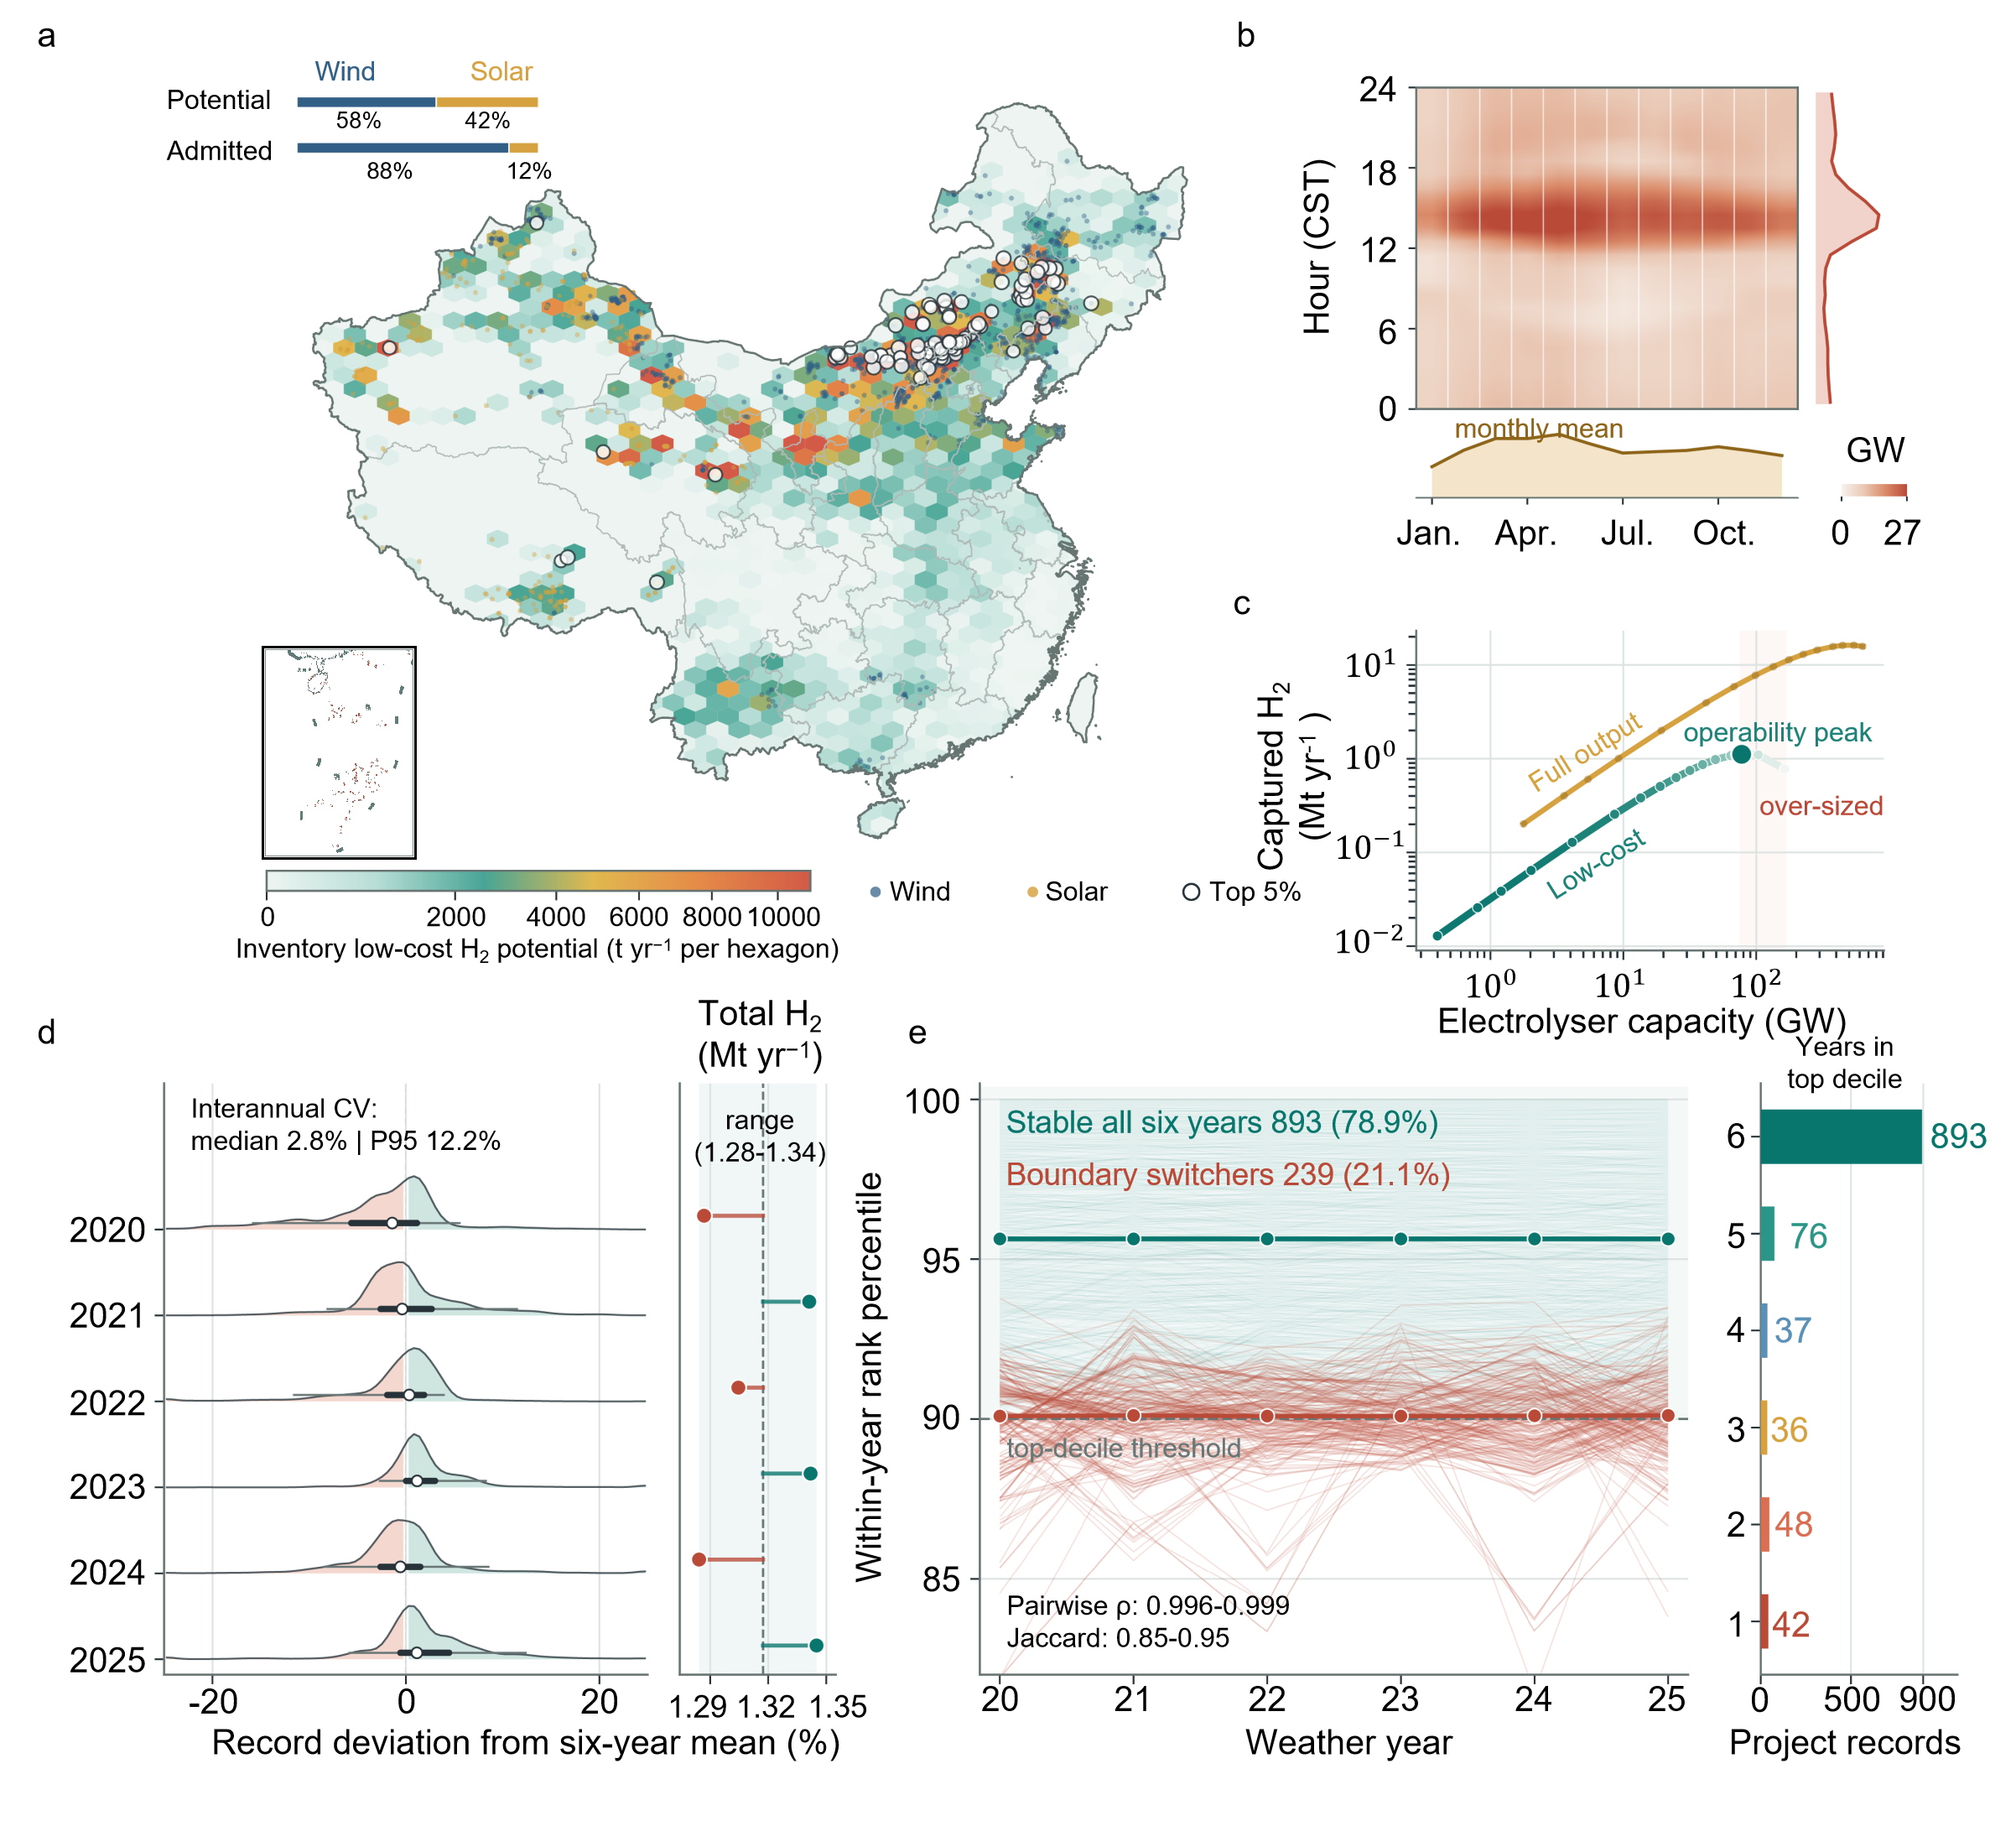
\includegraphics[width=\textwidth]{figures/Figure1_selected.png}
\caption{\textbf{Spatial, temporal and operating constraints delimit hydrogen production from low-opportunity-cost electricity within the project-record inventory.} \textbf{a}, Spatial distribution of hydrogen potential from system-constrained electricity; dark records meet the lower return criterion, open circles identify the top 5\% of admitted records ranked by annual hydrogen output, and stacked bars compare the wind--solar composition of physical potential and admitted production. Main-map coastline, land mask and visible administrative linework derive from OpenStreetMap (\copyright\ OpenStreetMap contributors) and share the station projection; the boxed South China Sea locator is a cleaned display derivative of standard-map product GS(2023)2767 and is not used analytically. The map colour scale is capped at the occupied-hexagon 97.5th percentile. \textbf{b}, Month--hour climatology with diurnal and seasonal margins; its colour scale is capped at the 98th percentile. \textbf{c}, Operating frontier for electrolyser capacity, realised hydrogen and active low-cost hours under the mutually exclusive constrained-electricity and full-output branches. \textbf{d}, Record-level deviations from six-year mean hydrogen potential and inventory totals for ERA5 weather years 2020--2025; the annotation reports the across-record distribution of interannual coefficients of variation. Density tails are clipped at $\pm25\%$ for display, while white points, thick lines and thin lines denote medians, interquartile ranges and 5th--95th percentiles calculated from the unclipped values. \textbf{e}, Rank trajectories and persistence among records in the top resource decile.}
\label{fig:resource}
\end{figure}

\begin{figure}[p]
\centering
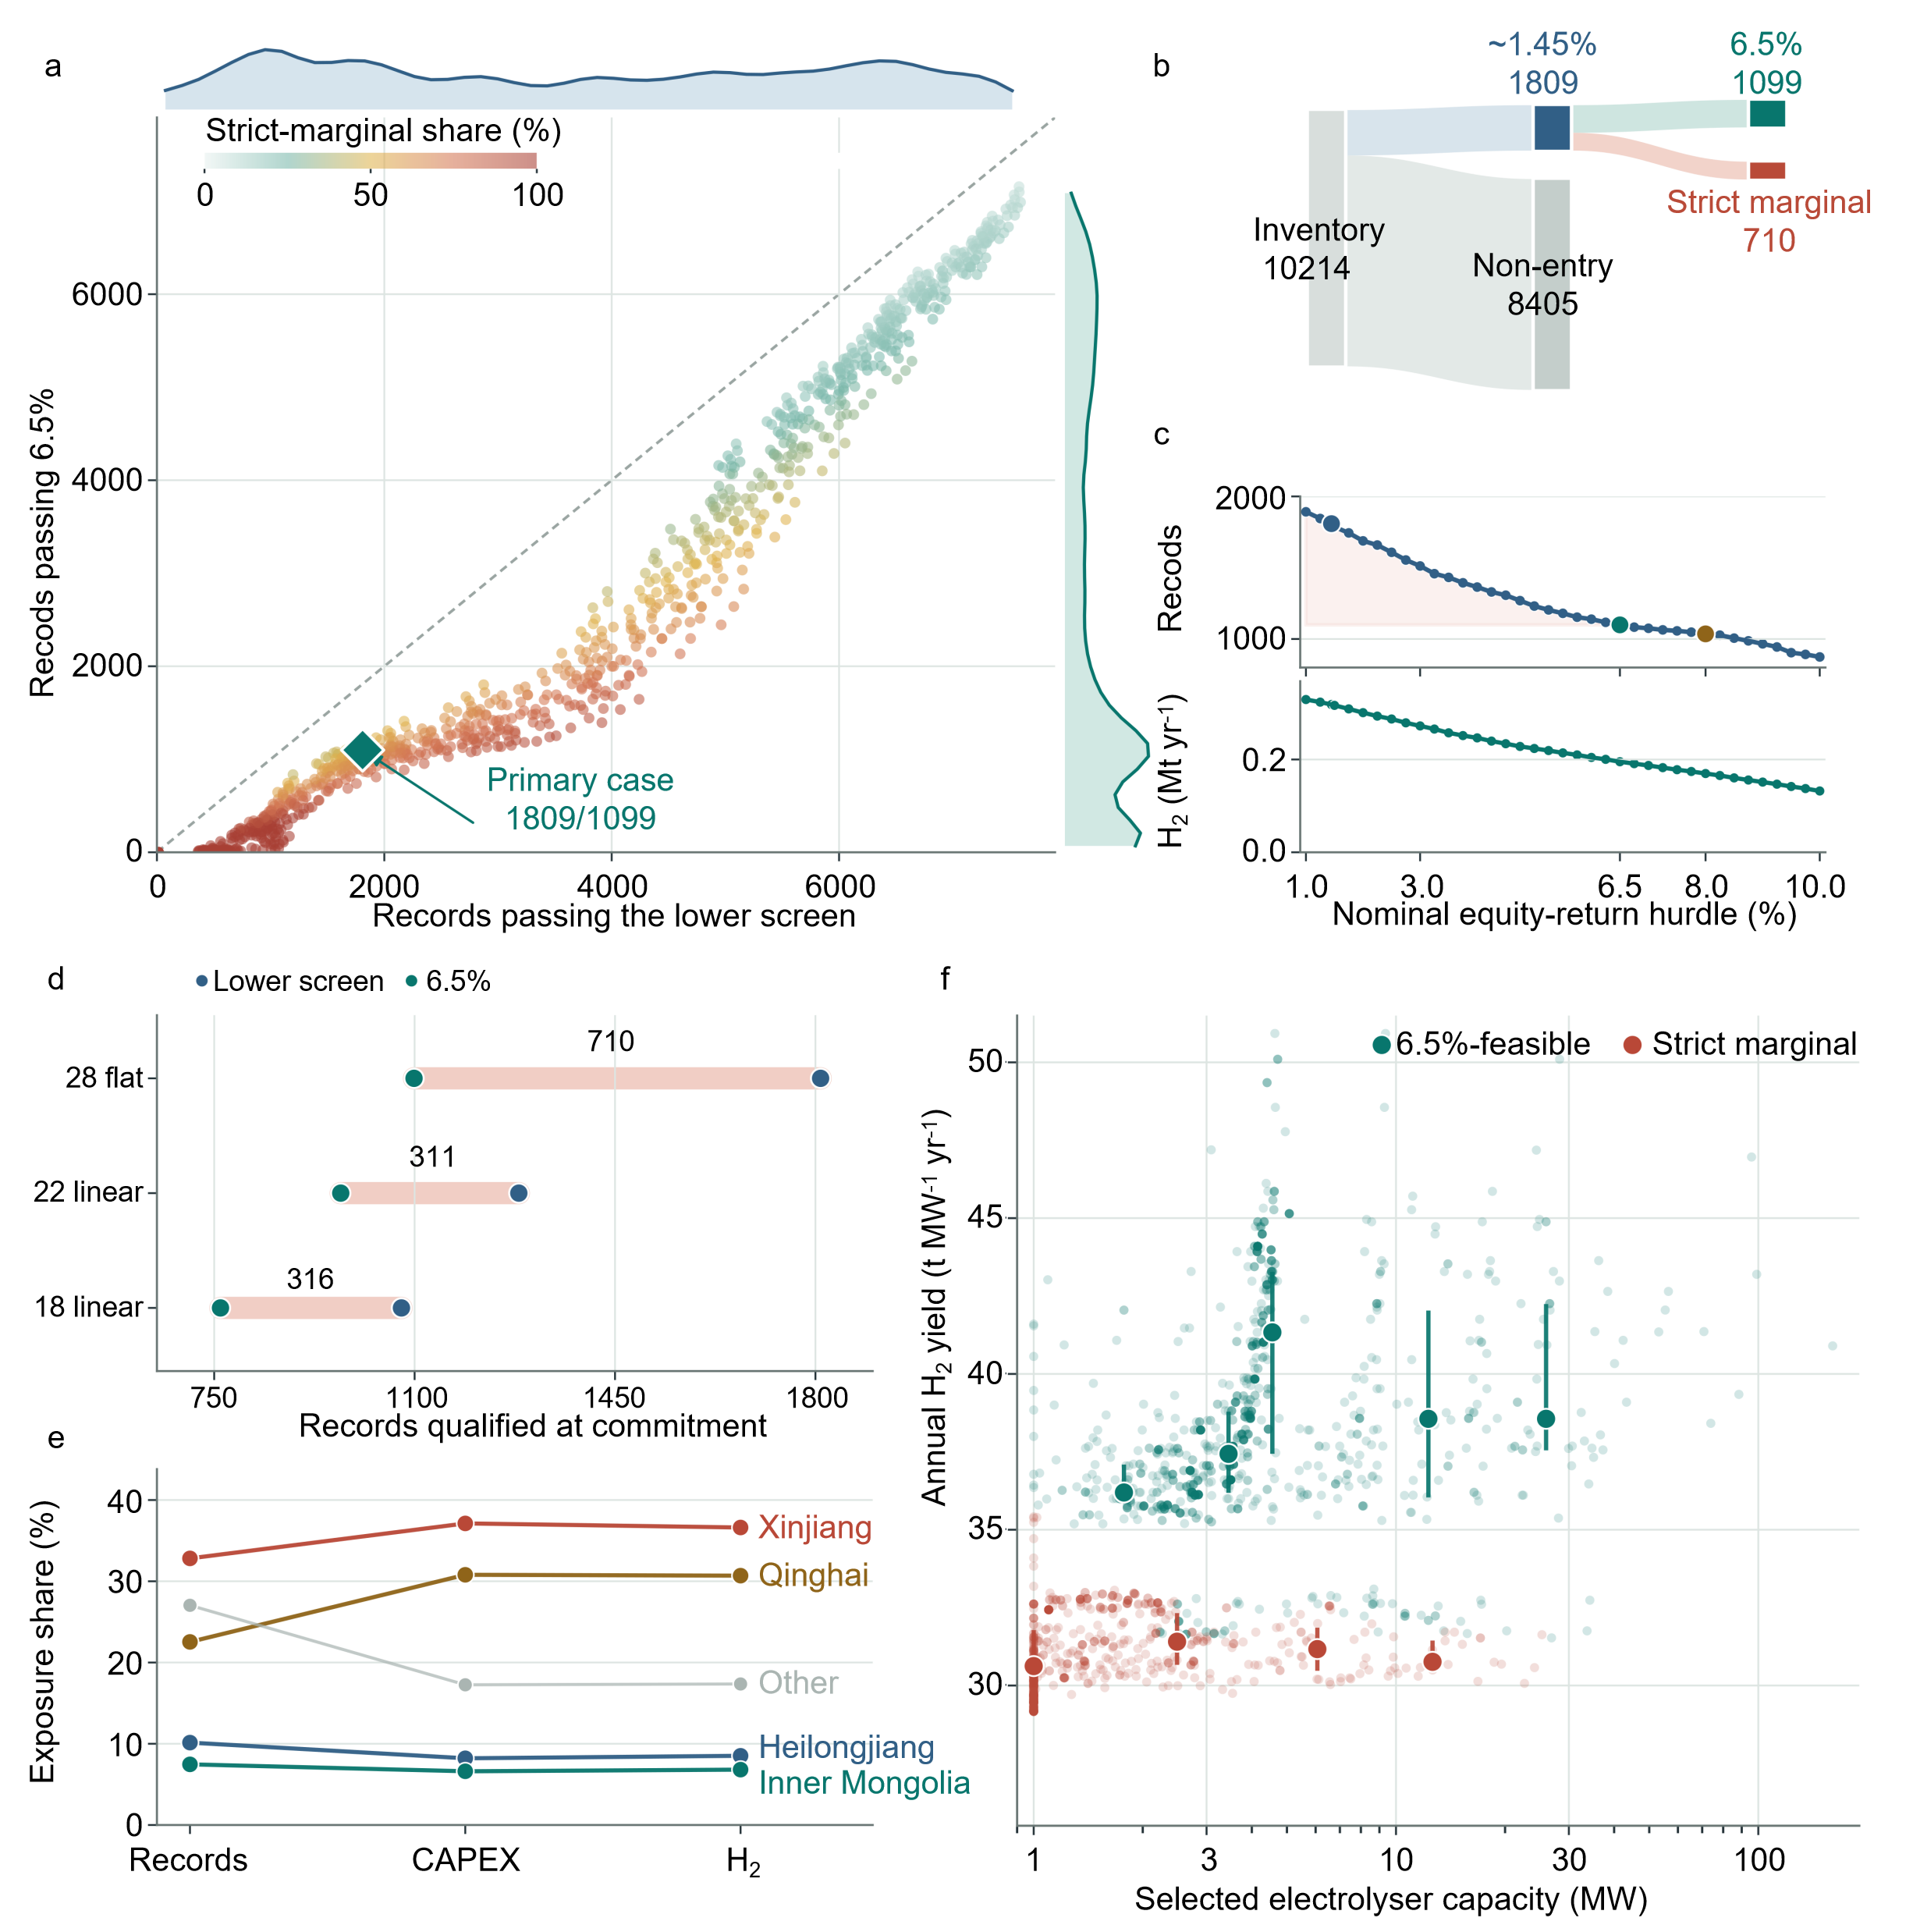
\includegraphics[width=0.98\textwidth]{figures/Figure2_selected.png}
\caption{\textbf{Return criteria create a continuous and information-dependent qualification boundary.} \textbf{a}, Records passing the lower and 6.5\% screens across 972 deterministic constrained-electricity configurations; colour gives the full 0--100\% strict-marginal share, marginal curves show the distributions and the diamond marks the primary case. The configurations are an unweighted sensitivity ensemble, not a probability distribution. \textbf{b}, Flow from the 10,214-record inventory to static lower-rule qualification, non-qualification, 6.5\%-qualified and strict-marginal cohorts. \textbf{c}, Qualified records and annual hydrogen after independent resizing across a continuous 1--10\% nominal equity-return frontier; highlighted points mark the lower rule, 6.5\% and 8\%. \textbf{d}, Paired qualification under a static 28~\cnykg{} reference and linear 22 and 18~\cnykg{} paths anticipated at commitment; coral spans give the strict-marginal cohort. \textbf{e}, Provincial shares of strict-marginal records, gross installed-system capital and annual hydrogen output. \textbf{f}, Record-level electrolyser capacity and annual hydrogen yield for 6.5\%-feasible and strict-marginal records. Large points and vertical intervals show unconnected medians and interquartile ranges in shared logarithmic bins; only bins containing at least 20 records are summarised.}
\label{fig:admission}
\end{figure}

\begin{figure}[p]
\centering
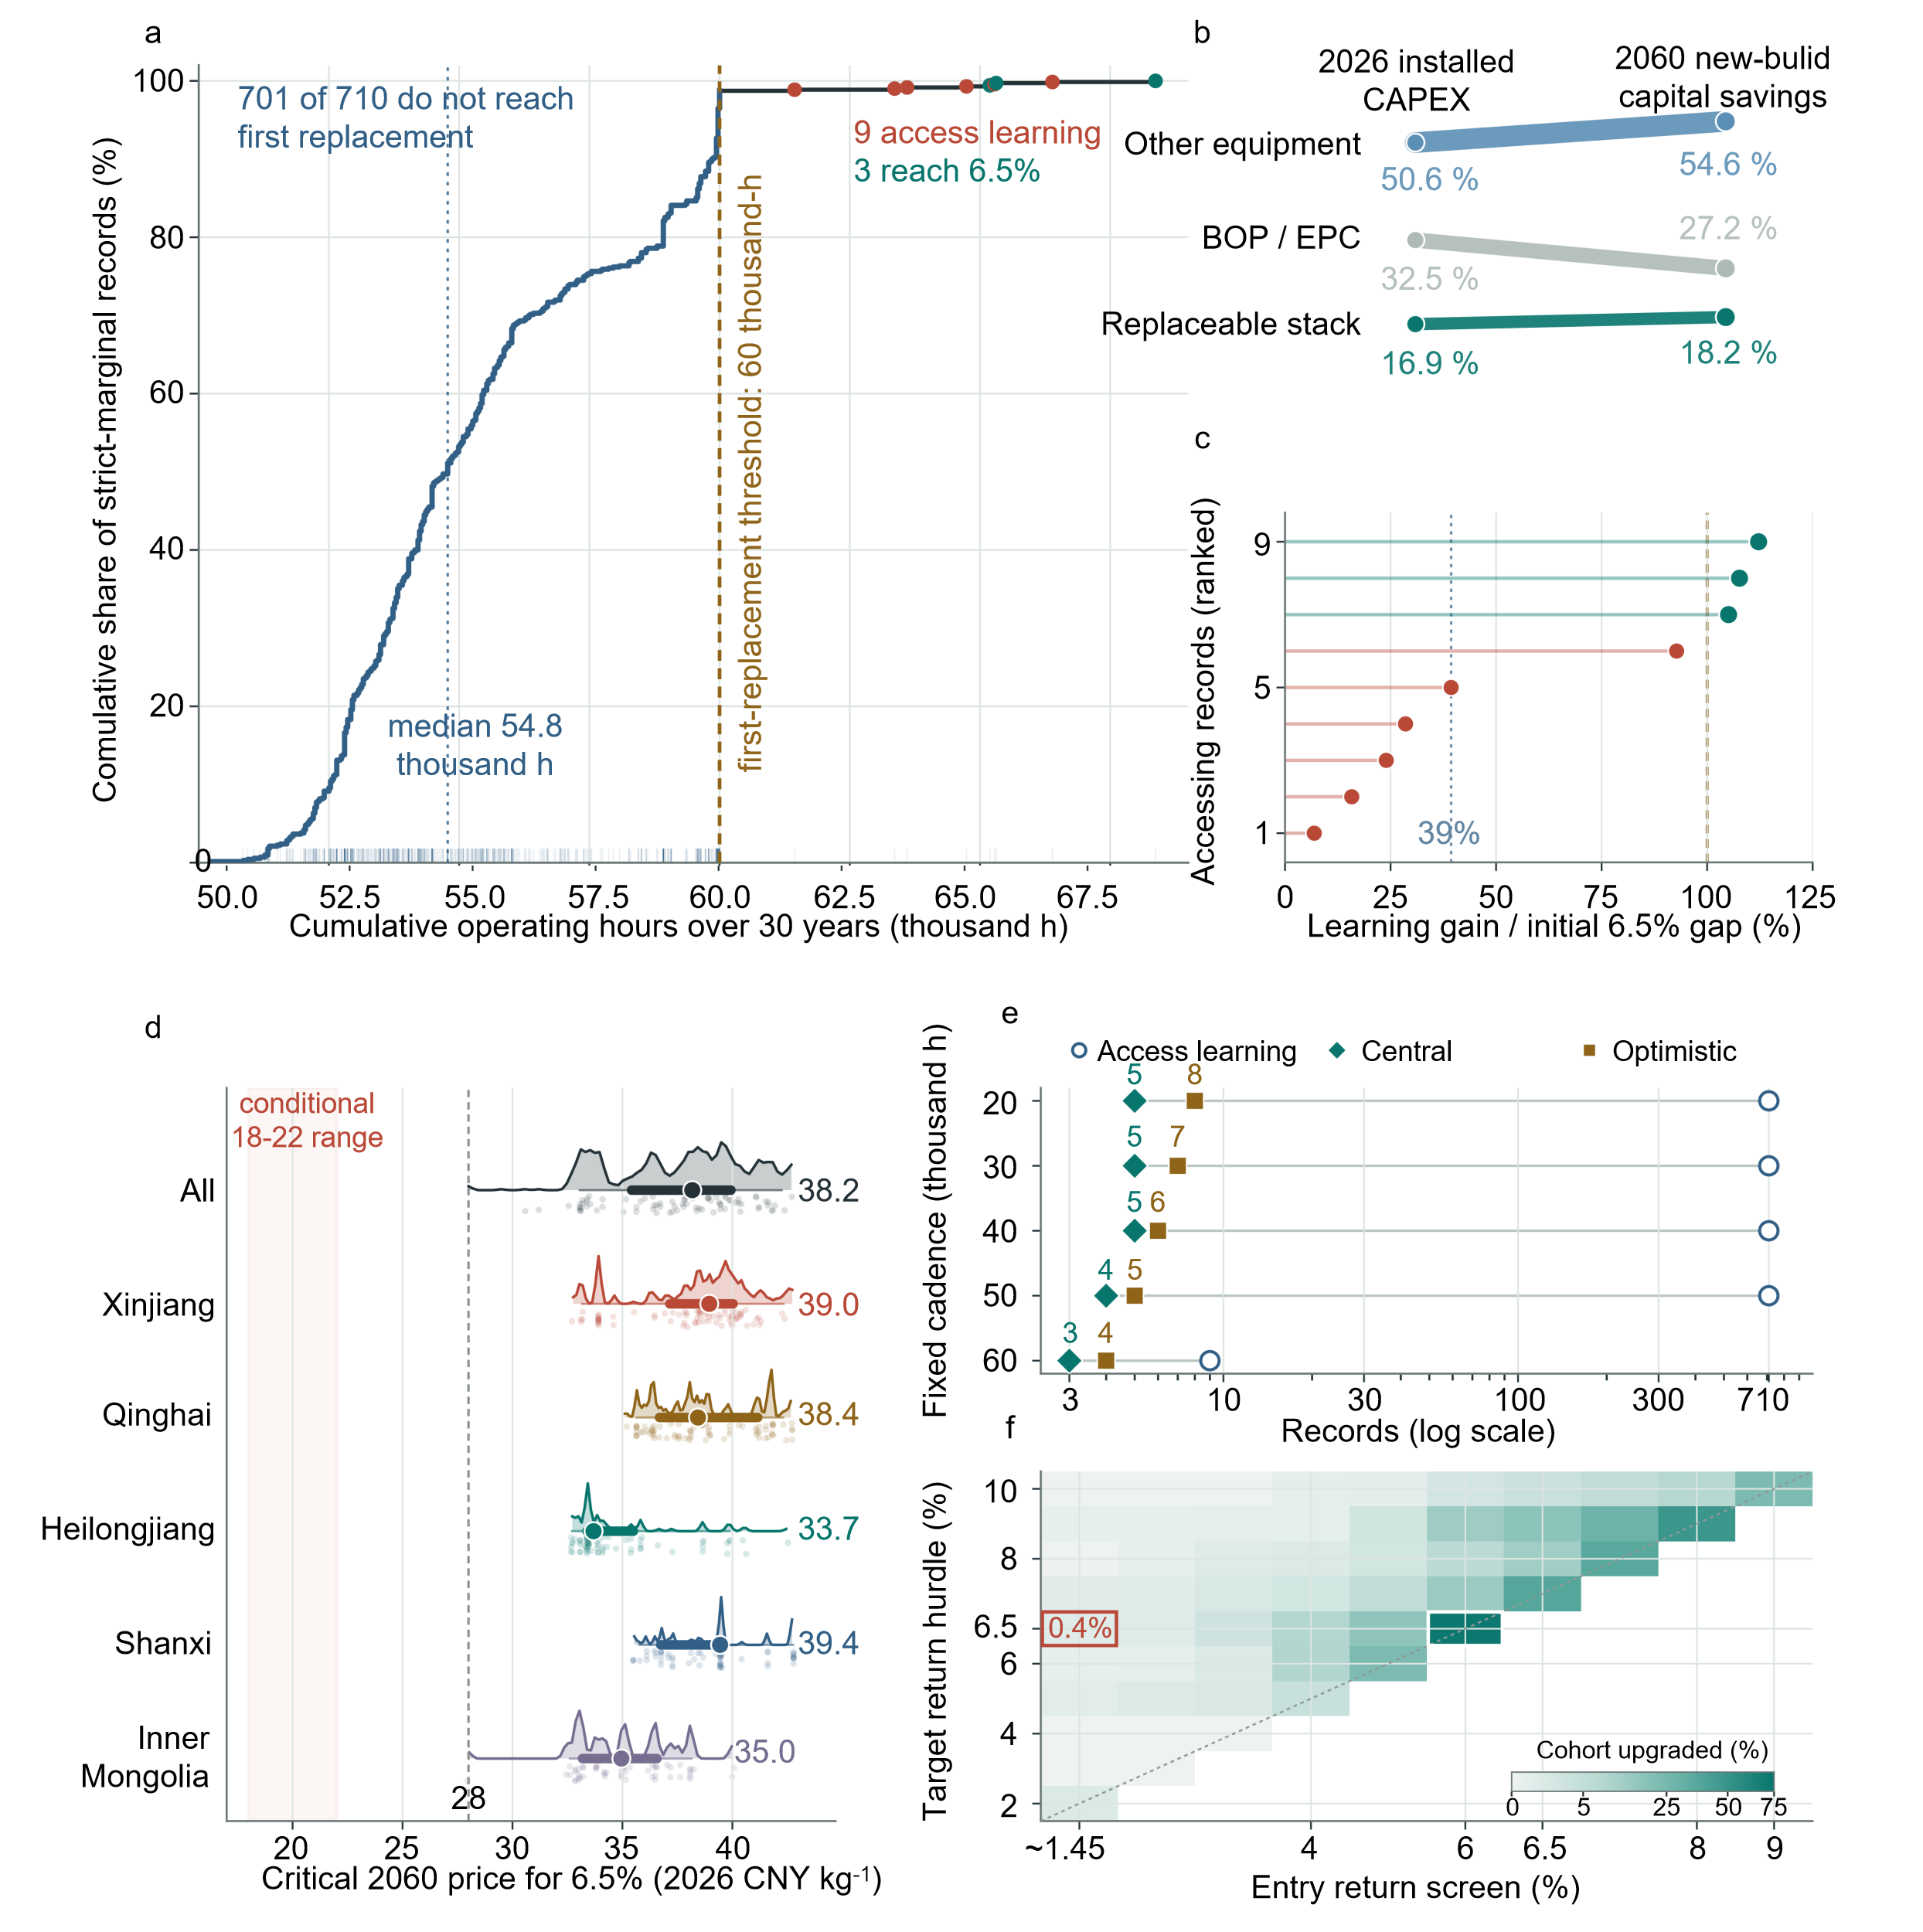
\includegraphics[width=\textwidth]{figures/Figure3_selected.png}
\caption{\textbf{Replacement access is necessary but insufficient for operating learning to repair incumbent returns.} \textbf{a}, Empirical cumulative distribution of 30-year operating hours across 710 strict-marginal records relative to the central 60,000-hour first-replacement threshold. The blue curve segment identifies records that do not trigger replacement; coral points identify six records that access learning but remain below 6.5\%, and teal points identify the three accessing records that close their initial 6.5\% NPV gaps. Three near-coincident observations retain their exact coordinates and are layered from left to right using a common display size. \textbf{b}, Change in the component shares of 2026 installed CAPEX and 2060 new-build capital savings; only the stack-embodied share is accessible to incumbents, and the displayed source-grounded component boundary spans 11.3--42.3\%. \textbf{c}, Share of each initial 6.5\% NPV gap closed by central operating learning among the nine records that trigger replacement, ranked by closure share; the vertical line at 100\% denotes complete closure. \textbf{d}, Distributions of the conditional 2060 terminal price required to reach 6.5\%, overall and in the principal exposed provinces; points, thick intervals and thin intervals denote medians, interquartile ranges and 5th--95th percentile ranges, respectively. \textbf{e}, Fixed-cadence falsification test comparing records that trigger replacement with records reaching 6.5\% under central and source-optimistic learning; at 20,000--50,000 hours all 710 records access learning but only four to eight upgrade. \textbf{f}, Flat-price return-screen surface across all 55 lower-to-higher criterion pairs. Cell colour gives the share of each locked marginal cohort upgraded by central operating learning; the outlined cells mark the approximately 1.45--6.5\% comparison and the narrow 6.0--6.5\% counterfactual.}
\label{fig:learning}
\end{figure}

\begin{figure}[p]
\centering
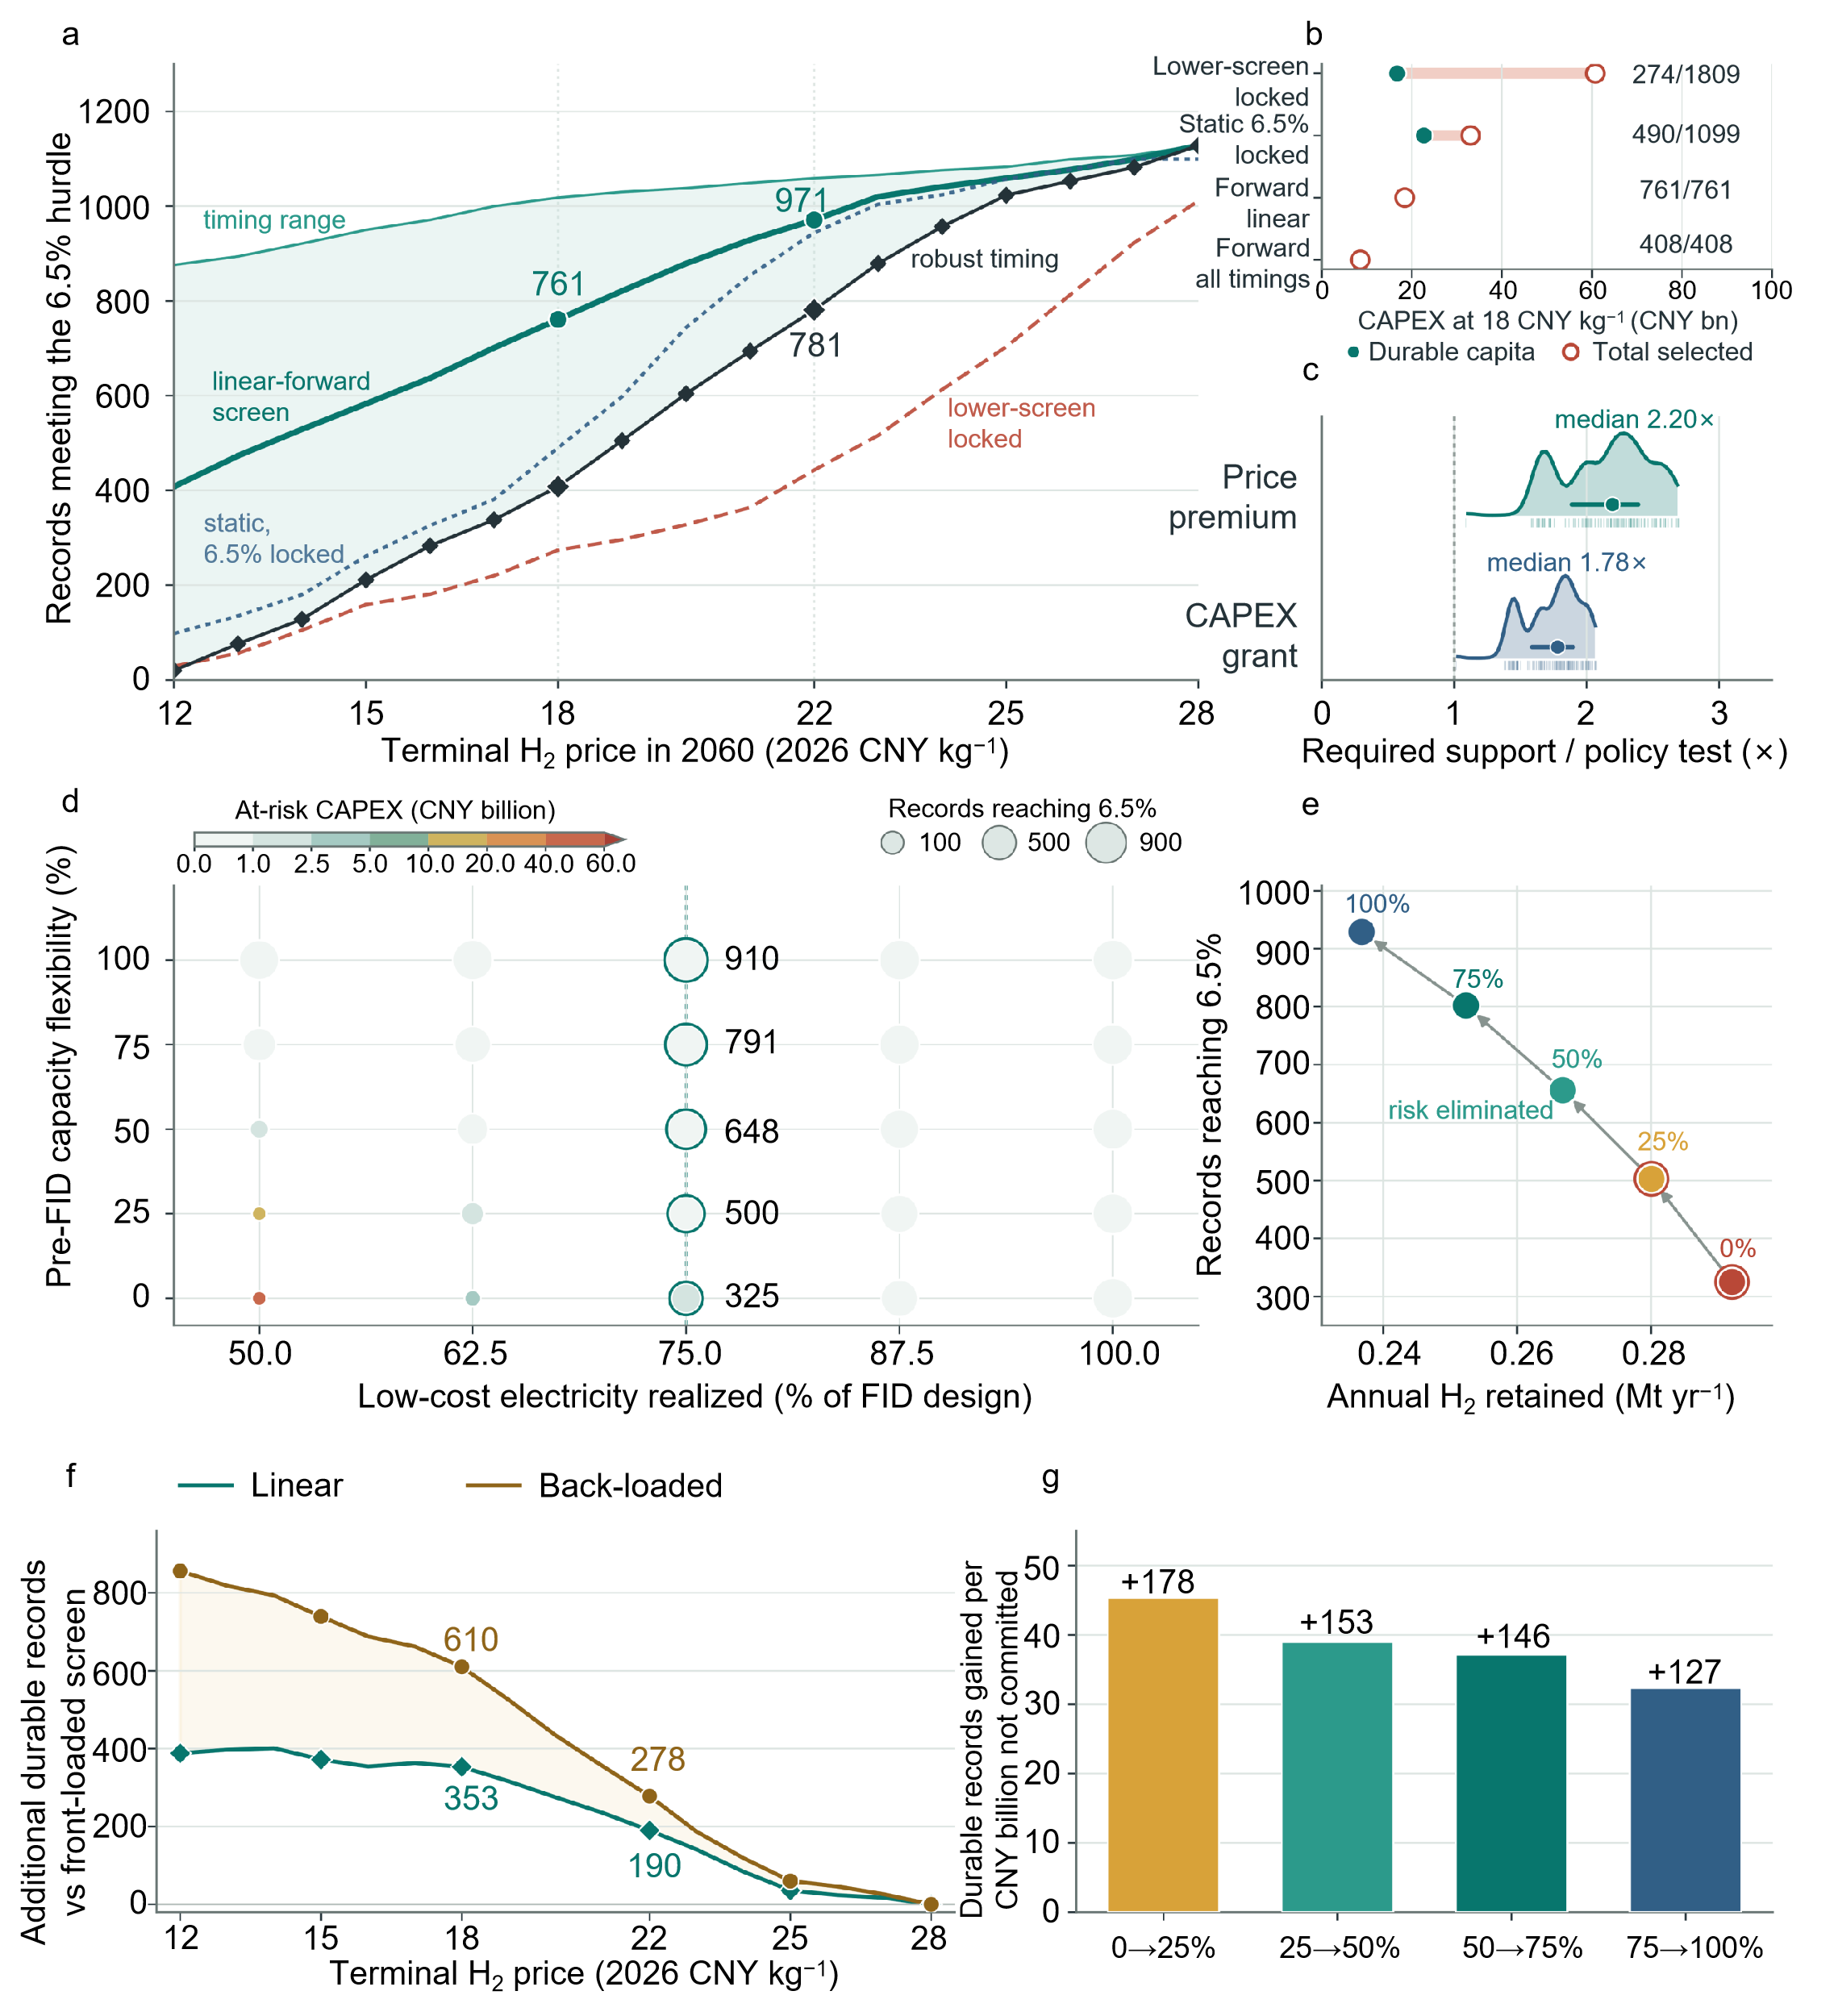
\includegraphics[width=0.98\textwidth]{figures/Figure4_selected.png}
\caption{\textbf{Price-informed screening and pre-investment capacity flexibility move exposure ahead of capital lock-in.} \textbf{a}, Records remaining above 6.5\% under alternative commitment rules across conditional terminal prices of 12--28~\cnykg{}; the green band spans front-loaded to back-loaded timing, the heavy line denotes the linear path and black diamonds denote timing-robust screening. \textbf{b}, Durable and total selected capital under four commitment rules for the linear 18~\cnykg{} path; right-hand labels give durable/selected records. \textbf{c}, Required 15-year price premiums and upfront capital grants normalised by illustrative policy tests; ridges show distributions, thick lines show interquartile ranges and circles mark medians. \textbf{d}, At-risk capital under the primary 1-MW minimum-build convention across resource realisation and pre-FID adjustability; colour gives at-risk capital, circle area gives records reaching 6.5\%, and outlines and adjacent values identify the 75\% resource slice. \textbf{e}, Continuous-downsizing trade-off at 75\% resource realisation between annual hydrogen retained and records reaching 6.5\%; labels give adjustability and coral outlines identify cases with residual exposure. \textbf{f}, Gain in durable records under linear and back-loaded timing relative to the worst-case front-loaded screen. Lines include every one-CNY endpoint from 12 to 28~\cnykg{}, and markers identify the six labelled endpoints. \textbf{g}, Marginal durability yield of each 25-percentage-point increase in continuous pre-FID adjustability at 75\% resource realisation. Each step releases the same 3.93\,billion CNY of planned CAPEX from commitment. Bars report the additional records reaching 6.5\% per CNY billion not committed, and labels above bars give the corresponding record gains; declining bar heights therefore indicate diminishing marginal durability gains per equal capital increment.}
\label{fig:screening}
\end{figure}

\clearpage
\setcounter{figure}{0}
\renewcommand{\figurename}{Extended Data Fig.}
\renewcommand{\thefigure}{\arabic{figure}}
\renewcommand{\theHfigure}{ED.\arabic{figure}}

\begin{figure}[p]
\centering
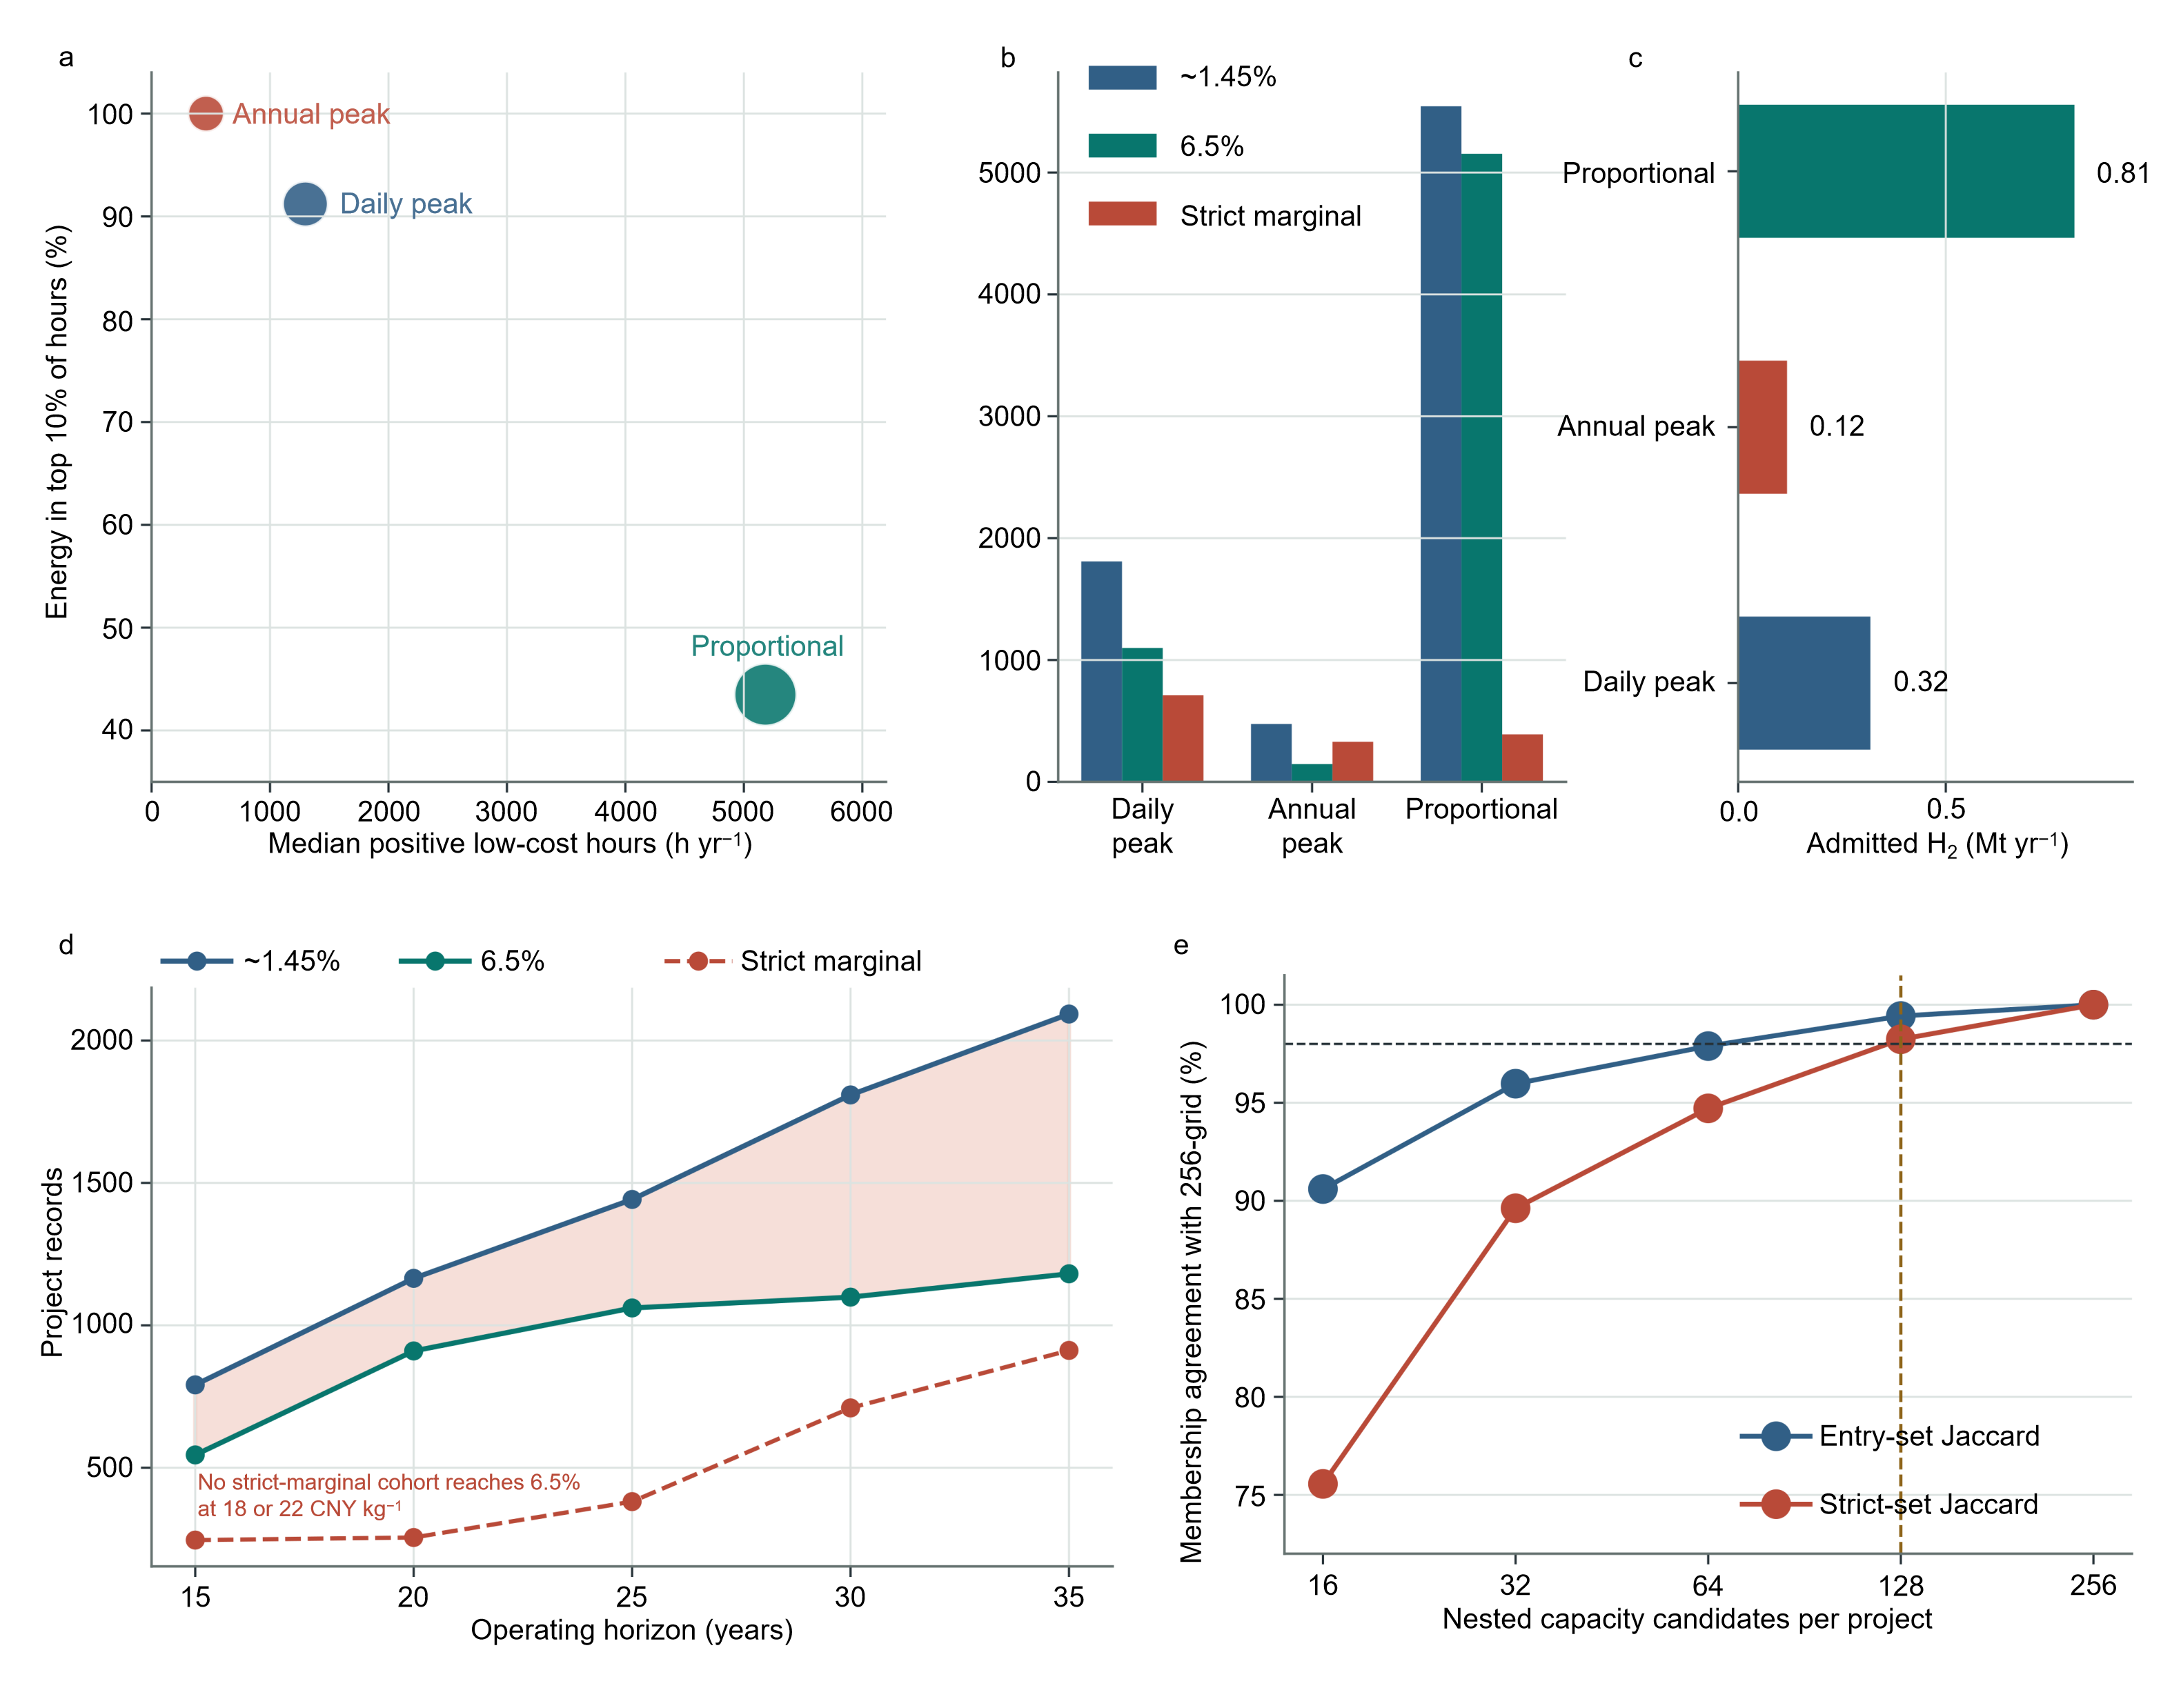
\includegraphics[width=\textwidth]{figures/ExtendedDataFigure1_selected.png}
\caption{\textbf{Hourly reconstruction, evaluation-horizon and capacity-search robustness.} \textbf{a--c}, Full-chain admission and strict-marginal outcomes under the daily peak-shaving, annual peak-shaving and proportional-allocation proxies; bubble area in \textbf{a} gives admitted hydrogen. \textbf{d}, Durable-return outcomes across 15--35-year evaluation horizons. \textbf{e}, Membership convergence across 16--256 nested capacity grids relative to the 256-grid reference. The vertical line identifies the 128-candidate main grid; insertion of the exact 1-MW boundary followed by adaptive local search reproduces the final entry and strict-marginal memberships with 100\% agreement. Exact project-record counts remain conditional on the hourly proxy, while the failure of strict-marginal cohorts to reach durable 6.5\% at terminal prices of 22~\cnykg{} or less is stable across the tested boundaries.}
\label{fig:extendedrobustness}
\end{figure}

\end{document}
